\documentclass[../main.tex]{subfiles}

\usepackage{nopageno} %Seitenzahlen auf richtiger Seite 

\usepackage[left=2cm, right=2cm, top=2cm, includehead, includefoot, headheight=17pt]{geometry}

\usepackage[utf8x]{inputenc}
\usepackage[english]{babel}
\usepackage{amsmath,amssymb,amsthm}
\usepackage{framed}
\usepackage{wasysym}
\usepackage[T1]{fontenc} %Silbentrennung 
\usepackage{color} %Farbe
\usepackage{graphicx}
\usepackage{float}%Grafik am gleichen Ort plazieren
%pdf. png. einfach eingliedern
\usepackage{subfigure} %Grafiken nebeneinander
\usepackage{pdfpages}
\usepackage{ulem} 	%\uuline{urgent}    % doppelt unterstreichen
%\uwave{boat}      % unterschlängeln
%\sout{wrong}       % durchstreichen
%\xout{removed}     % ausstreichen mit //////.

\usepackage{tikz}
\usetikzlibrary{trees}
\usetikzlibrary{plotmarks}
\usetikzlibrary{angles,quotes,babel}
\usetikzlibrary{shadings}
\usetikzlibrary{patterns}
\usetikzlibrary{matrix}
\usetikzlibrary{arrows}
\usetikzlibrary{calc}

\usepackage{pgfplots}
\usepackage{pgf-pie}
\pgfplotsset{compat=1.10}
\usepgfplotslibrary{statistics}
\usepgfplotslibrary{fillbetween}

\usepackage{tkz-euclide}
\usepackage{enumerate}
\usepackage{stmaryrd}
\usepackage{tabularx}
\usepackage{wrapfig}
\usepackage{epsdice}
\usepackage{multirow}
\usepackage{rotating}
\usepackage{pdflscape}
\usepackage{fancyhdr}

\pagestyle{fancy} %eigener Seitenstil
\fancyhf{} %alle Kopf- und Fußzeilenfelder bereinigen
\fancyhead[L]{} %Kopfzeile links
\fancyhead[C]{} %zentrierte Kopfzeile
\fancyhead[R]{} %Kopfzeile rechts
\renewcommand{\headrulewidth}{0.4pt} %obere Trennlinie
\fancyfoot[C]{\thepage} %Seitennummer
\renewcommand{\footrulewidth}{0.4pt} %untere Trennlinie

% Number spaces 
\newcommand{\CC}{\ensuremath{\mathbb{C}}}
\newcommand{\RR}{\ensuremath{\mathbb{R}}}
\newcommand{\QQ}{\ensuremath{\mathbb{Q}}}
\newcommand{\ZZ}{\ensuremath{\mathbb{Z}}}
\newcommand{\NN}{\ensuremath{\mathbb{N}}}
\newcommand{\LL}{\ensuremath{\mathbb{L}}}
\newcommand{\DD}{\ensuremath{\mathbb{D}}}
\newcommand{\WW}{\ensuremath{\mathbb{W}}}

%draw chemestry molecules 
\usepackage{chemfig} % https://mirror.ox.ac.uk/sites/ctan.org/macros/generic/chemfig/

\newcommand\vv[1]{%
	\begin{tikzpicture}[baseline=(arg.base)]
		\node[inner xsep=0pt] (arg) {$#1$};
		\draw[line cap=round,line width=0.45,->,shorten >= 0.2pt, shorten <= 0.7pt] (arg.north west) -- (arg.north east);
	\end{tikzpicture}%
} %command will render \vv{x} with an arrow aboth 

\renewcommand{\labelenumi}{\roman{enumi})}

\DeclareMathOperator{\ggT}{ggT}
\DeclareMathOperator{\sign}{sign}

%sections
\theoremstyle{plain}
\newtheorem{Thm}{Theorem}[section]
\newtheorem{Def}[Thm]{Definition}
\newtheorem{Prop}[Thm]{Proposition}

\theoremstyle{definition}
\newtheorem{lemma}[Thm]{Lemma}
\newtheorem{corollary}[Thm]{Corollary}
\newtheorem{claim}[Thm]{Claim}
\newtheorem{Proof}[Thm]{Proof}
\newtheorem{Ex}[Thm]{Example}

\newtheorem{Exercise}{ex}[section] %follow proper enum
\newtheorem{ex}[Exercise]{Exercise}
\newtheorem{Solution}{sol}[section]
\newtheorem{sol}[Solution]{Solution}

\theoremstyle{remark}
\newtheorem{remark}[Thm]{Remark} % follows thm enum

\newtheorem{comment}{Comment}[section] %follow comment enum
\newtheorem{notation}[comment]{Notation}
\newtheorem{reasoning}[comment]{Reasoning}
\newtheorem{Intpr}[comment]{Interpretation}

%some premmade with title (uterwise use \textbf{Title} ...)
\newenvironment{ThmWithTitle}[1]{%
	\begin{Thm}[\textbf{#1}]}{\end{Thm}}
\newenvironment{PropWithTitle}[1]{%
	\begin{Prop}[\textbf{#1}]}{\end{Prop}}
\newenvironment{ExWithTitle}[1]{%
	\begin{Ex}[\textbf{#1}]}{\end{Ex}}
\newenvironment{DefWithTitle}[1]{%
	\begin{Def}[\textbf{#1}]}{\end{Def}}
\newenvironment{RemarkWithTitel}[1]{%
	\begin{remark}[\textbf{#1}]}{\end{remark}}

%format of paragraph 
\renewcommand\paragraph{\@startsection{paragraph}{4}{\z@}%
	{-2.5ex\@plus -1ex \@minus -.25ex}%
	{1.25ex \@plus .25ex}%
	{\normalfont\normalsize\bfseries}}
\makeatother
\setcounter{secnumdepth}{4} % how many sectioning levels to assign numbers to
\setcounter{tocdepth}{4}    % how many sectioning levels to show in ToC

\newcounter{row} 
\renewcommand\therow{\alph{row}} %hier a,b,c etc. def und mit therow abrufbar

\newenvironment{aufz}
{\setcounter{row}{0}%
	\par\noindent\tabularx{\linewidth}[t]
	{\cdot{20}{>{\stepcounter{row}\makebox[1.5em][l]{\therow)\hfill}}X}} %bis max 20 Elemente nebeinander
}
{\endtabularx}


%biblio
\usepackage[]{biblatex}
\addbibresource{referenzenma.bib} 

%glossary
\usepackage{glossaries}
\usepackage{import}


\usepackage{rotating} % Include this package in the preamble

%\newglossaryentry{Enzyme}{
	name={Enzyme},
	description={A macromolecular biological catalyst that significantly accelerates chemical reactions, often with high specificity. They can be proteins or catalytically active RNA molecules:contentReference[oaicite:0]{index=0}.}
}

\newglossaryentry{Cofactor}{
	name={Cofactor},
	description={An inorganic chemical component required for enzyme activity. Often metal ions such as Fe\textsuperscript{2+}, Mg\textsuperscript{2+}, or Zn\textsuperscript{2+}:contentReference[oaicite:1]{index=1}.}
}

\newglossaryentry{Coenzyme}{
	name={Coenzyme},
	description={A complex organic or metallorganic molecule required for enzyme function, often derived from vitamins. Acts as a transient carrier of specific functional groups:contentReference[oaicite:2]{index=2}.}
}

\newglossaryentry{Systematic name}{
	name={Systematic name},
	description={A precise name given to an enzyme that indicates the substrates and type of reaction it catalyzes (e.g., ATP:glucose phosphotransferase for hexokinase):contentReference[oaicite:3]{index=3}.}
}

\newglossaryentry{Classification number}{
	name={Classification number},
	description={A four-part code assigned to enzymes based on the type of reaction they catalyze (e.g., 2.7.1.1 for hexokinase):contentReference[oaicite:4]{index=4}.}
}

\newglossaryentry{Activation Energy}{
	name={Activation Energy},
	description={The energy barrier ($$\Delta G^{\ddagger}$$) between the ground state and the transition state that must be overcome for a reaction to proceed:contentReference[oaicite:5]{index=5}.}
}

\newglossaryentry{Transition State Theory}{
	name={Transition State Theory},
	description={A model describing the top of the energy hill in a reaction coordinate where reactants are equally likely to proceed to products or return to reactants. Not to be confused with reaction intermediates:contentReference[oaicite:6]{index=6}.}
}

\newglossaryentry{Transition State}{
	name={Transition State},
	description={The highest-energy configuration along the reaction coordinate. It is the point at which the system is equally likely to proceed toward products or return to reactants. It is not a stable intermediate and is denoted as $\ddagger$:contentReference[oaicite:0]{index=0}.}
}


\newglossaryentry{Reaction Intermediate}{
	name={Reaction Intermediate},
	description={A short-lived, chemically distinct species that occurs during the transformation of reactants to products, such as enzyme-substrate (ES) complexes:contentReference[oaicite:7]{index=7}.}
}

\newglossaryentry{K_{eq}}{
	name={$K_{eq}$},
	description={The equilibrium constant of a reaction, given by the ratio $$\frac{[P]}{[S]}$$. Not affected by enzymes:contentReference[oaicite:8]{index=8}.}
}

\newglossaryentry{Delta G}{
	name={$\Delta G$},
	description={The change in free energy during a reaction. $\Delta G°$ refers to standard conditions, and $\Delta G°^{\prime}$ includes biochemical conditions (pH = 7):contentReference[oaicite:9]{index=9}.}
}

\newglossaryentry{Delta G dagger}{
	name={$\Delta$ $G^{\ddagger}$},
	description={The activation free energy, the difference in energy between the ground state and the transition state:contentReference[oaicite:10]{index=10}.}
}

\newglossaryentry{Return Rate}{
	name={Return Rate},
	description={The rate of the reaction based on substrate concentration and a rate constant $$k$$, where $$v = k[S]$$:contentReference[oaicite:11]{index=11}.}
}

\newglossaryentry{Catalytic Power}{
	name={Catalytic Power},
	description={The ability of enzymes to lower the activation energy and provide alternate reaction pathways, enhancing the reaction rate:contentReference[oaicite:12]{index=12}.}
}

\newglossaryentry{Active Site}{
	name={Active Site},
	description={The region of the enzyme where substrate binding and catalysis occur, often through specific amino acid residues:contentReference[oaicite:13]{index=13}.}
}

\newglossaryentry{Transition State Complementarity}{
	name={Transition State Complementarity},
	description={The enzyme binds more tightly to the transition state than to the substrate, thereby lowering the activation energy and enhancing catalysis:contentReference[oaicite:14]{index=14}.}
}

\newglossaryentry{Rate Enhancement}{
	name={Rate Enhancement},
	description={The increase in reaction speed due to the lowering of the activation energy by enzyme catalysis:contentReference[oaicite:15]{index=15}.}
}

\newglossaryentry{Binding}{
	name={Binding},
	description={The specific interaction between enzyme and substrate, often involving multiple weak noncovalent interactions to drive catalysis:contentReference[oaicite:16]{index=16}.}
}

\newglossaryentry{Specificity}{
	name={Specificity},
	description={The enzyme's ability to select exact substrates and catalyze a specific reaction, influenced by binding energy and structural complementarity:contentReference[oaicite:17]{index=17}.}
}

\newglossaryentry{Acid-Base Catalysis}{
	name={Acid-Base Catalysis},
	description={A catalytic mechanism in which amino acid residues act as proton donors or acceptors to stabilize charged intermediates, increasing reaction rates when water alone is insufficient:contentReference[oaicite:0]{index=0}.}
}

\newglossaryentry{Covalent Catalysis}{
	name={Covalent Catalysis},
	description={A mechanism where the enzyme forms a transient covalent bond with the substrate, creating an alternative reaction pathway with lower activation energy. This requires nucleophilic groups on the enzyme:contentReference[oaicite:1]{index=1}.}
}

\newglossaryentry{Metal Ion Catalysis}{
	name={Metal Ion Catalysis},
	description={Catalysis involving metal ions that can stabilize negative charges on reaction intermediates, help substrate orientation, or mediate redox reactions through reversible changes in oxidation state:contentReference[oaicite:2]{index=2}.}
}

\newglossaryentry{Enzyme Kinetics}{
	name={Enzyme Kinetics},
	description={The study of the rate of enzyme-catalyzed reactions and how they change in response to experimental parameters like substrate concentration:contentReference[oaicite:3]{index=3}.}
}

\newglossaryentry{v_0}{
	name={$v_0$},
	description={The initial velocity of an enzyme-catalyzed reaction, measured at the very beginning before product accumulates. At low $[S]$, $v_0$ increases almost linearly with $[S]$:contentReference[oaicite:4]{index=4}.}
}

\newglossaryentry{Enzyme Saturation}{
	name={Enzyme Saturation},
	description={The condition where increasing substrate concentration no longer increases the reaction rate because all active sites are occupied, resulting in a plateau at $v_{max}$:contentReference[oaicite:5]{index=5}.}
}

\newglossaryentry{v_{max}}{
	name={$v_{max}$},
	description={The maximal velocity of an enzyme-catalyzed reaction when all enzyme molecules are saturated with substrate. Defined by $v_{max} = k_{cat}[E]_T$:contentReference[oaicite:6]{index=6}.}
}

\newglossaryentry{Michaelis-Menten}{
	name={Michaelis-Menten},
	description={A kinetic model describing enzyme activity: $v_0 = \frac{v_{max}[S]}{K_m + [S]}$, where $K_m$ is the substrate concentration at half-maximal velocity:contentReference[oaicite:7]{index=7}.}
}

\newglossaryentry{Lineweaver-Burk}{
	name={Lineweaver-Burk},
	description={A double reciprocal plot of enzyme kinetics: $\frac{1}{v_0} = \frac{K_m}{v_{max}} \cdot \frac{1}{[S]} + \frac{1}{v_{max}}$, used to linearize the Michaelis-Menten equation for easier interpretation:contentReference[oaicite:8]{index=8}.}
}

\newglossaryentry{Enzyme Efficiency}{
	name={Enzyme Efficiency},
	description={Measured by the specificity constant $\frac{k_{cat}}{K_m}$, which reflects both substrate binding and catalytic turnover. The theoretical upper limit is $10^8$ to $10^9 \text{ M}^{-1}\text{s}^{-1}$:contentReference[oaicite:9]{index=9}.}
}

\newglossaryentry{Inhibition}{
	name={Inhibition},
	description={The decrease or complete loss of enzyme activity due to the binding of a molecule (an inhibitor) that interferes with catalysis. Inhibition is fundamental to drug action and metabolic regulation:contentReference[oaicite:0]{index=0}.}
}

\newglossaryentry{Reversible Inhibition}{
	name={Reversible Inhibition},
	description={Inhibition where the inhibitor binds non-covalently and can dissociate from the enzyme. Includes competitive, non-competitive, and uncompetitive mechanisms:contentReference[oaicite:1]{index=1}.}
}

\newglossaryentry{Competitive Inhibitor}{
	name={Competitive Inhibitor},
	description={A molecule that competes with the substrate for binding at the active site. It increases $K_m$ but does not affect $v_{max}$:contentReference[oaicite:2]{index=2}.}
}

\newglossaryentry{Non-competitive Inhibitor}{
	name={Non-competitive Inhibitor},
	description={Binds to a site other than the active site and reduces the effective concentration of active enzyme. It decreases $v_{max}$ without changing $K_m$:contentReference[oaicite:3]{index=3}.}
}

\newglossaryentry{Uncompetitive Inhibitor}{
	name={Uncompetitive Inhibitor},
	description={Binds only to the enzyme-substrate complex, preventing product formation. It decreases both $v_{max}$ and $K_m$:contentReference[oaicite:4]{index=4}.}
}

\newglossaryentry{Irreversible Inhibition}{
	name={Irreversible Inhibition},
	description={Inhibition where the inhibitor covalently binds or permanently inactivates the enzyme, preventing further catalytic activity:contentReference[oaicite:5]{index=5}.}
}

\newglossaryentry{Suicide Inhibition}{
	name={Suicide Inhibition},
	description={A special type of irreversible inhibition where the enzyme converts the inhibitor into a reactive intermediate that covalently modifies and inactivates the enzyme:contentReference[oaicite:6]{index=6}.}
}

\newglossaryentry{Transition-State Analogs}{
	name={Transition-State Analogs},
	description={Stable molecules that resemble the transition state of a substrate and bind tightly to the enzyme, acting as potent inhibitors by exploiting transition state complementarity:contentReference[oaicite:7]{index=7}.}
}




\makeglossaries
\newglossaryentry{BP230}{
	name={BP230},
	description={A hemidesmosomal protein that connects plectin and keratin filaments to integrins in epithelial cells.}
}

\newglossaryentry{Ca2}{
	name={Ca2+},
	description={Calcium ions essential for cadherin-mediated adhesion by stabilizing cadherin domains and preventing molecular flexibility.}
}

\newglossaryentry{Collagenfibrils}{
	name={Collagen fibrils},
	description={Bundles of collagen molecules aligned in a staggered fashion, forming the structural framework of connective tissues.}
}

\newglossaryentry{EGFepidermalgrowthfactor}{
	name={EGF},
	description={A cell biology concept related to EGF (epidermal growth factor), requiring further specification.}
}

\newglossaryentry{integrin}{
	name={Integrin},
	description={A family of transmembrane receptors that mediate cell adhesion to the extracellular matrix and other cells. They link the cytoskeleton to the ECM and transmit bidirectional signals to regulate cell shape, motility, and survival.}
}

\newglossaryentry{EMT}{
	name={EMT},
	description={Epithelial-to-mesenchymal transition, a process where epithelial cells lose adhesion and gain migratory, invasive properties.}
}

\newglossaryentry{FN1}{
	name={FN1},
	description={One of the repeating domains in fibronectin responsible for collagen and fibrin binding.}
}

\newglossaryentry{FN2}{
	name={FN2},
	description={A fibronectin domain that contributes to binding interactions within the ECM.}
}

\newglossaryentry{FN3}{
	name={FN3},
	description={A fibronectin domain that contains the RGD motif for integrin binding, crucial for cell adhesion.}
}

\newglossaryentry{useless}{
	name={GPCR},
	description={G-protein-coupled receptor; activates intracellular signaling cascades including those that lead to integrin activation.}
}

\newglossaryentry{GTPase}{
	name={GTPase},
	description={A family of enzymes that hydrolyze GTP and regulate many signaling pathways, including cell adhesion and migration.}
}

\newglossaryentry{GTPaseRac}{
	name={GTPase Rac},
	description={A small GTPase that promotes actin polymerization and junction expansion during early cell-cell adhesion.}
}

\newglossaryentry{GTPaseRho}{
	name={GTPase Rho},
	description={A GTPase that promotes actomyosin contractility and maturation of adherens junctions into linear actin bundles.}
}

\newglossaryentry{Gapjunctions}{
	name={Gap junctions},
	description={Specialized intercellular connections composed of connexons that allow direct cytoplasmic exchange of small molecules and ions between neighboring cells.}
}

\newglossaryentry{Golgiapparatus}{
	name={Golgi apparatus},
	description={A cell organelle where glycosylation and processing of ECM proteins like procollagen occur before secretion.}
}

\newglossaryentry{hydroxylysyl}{
	name={Hydroxylysyl (Hyl)},
	description={A hydroxylated derivative of lysine found in collagen. It plays a critical role in forming covalent cross-links between collagen molecules, enhancing tensile strength of the extracellular matrix.}
}

\newglossaryentry{IGFBPInsulingrowthbindingfactor}{
	name={IGFBP},
	description={Insulin growth binding factor, a protein domain found in ECM components that binds insulin-like growth factors, modulating their availability and activity.}
}

\newglossaryentry{Integrin}{
	name={Integrin},
	description={A family of transmembrane receptors that link ECM proteins to the cytoskeleton and mediate bidirectional signaling.}
}

\newglossaryentry{Laminin}{
	name={Laminin},
	description={A cell biology concept related to Laminin, requiring further specification.}
}

\newglossaryentry{Laminin111}{
	name={Laminin-111},
	description={A trimeric laminin isoform found mainly in embryonic tissues, composed of α1, β1, and γ1 chains, crucial for basement membrane structure.}
}

\newglossaryentry{MET}{
	name={MET},
	description={Mesenchymal-to-epithelial transition, where mesenchymal cells adopt epithelial characteristics and form structured tissues.}
}

\newglossaryentry{Phosphoinositide}{
	name={Phosphoinositide},
	description={A lipid component of the membrane that binds Talin and other proteins to regulate integrin activation.}
}

\newglossaryentry{RIAM}{
	name={RIAM},
	description={An adaptor protein that helps recruit Talin to the plasma membrane during integrin activation.}
}

\newglossaryentry{Rap1}{
	name={Rap1},
	description={A small GTPase involved in inside-out signaling to activate integrins during processes like platelet adhesion.}
}

\newglossaryentry{Slug}{
	name={Slug},
	description={Slug is a transcription factor that regulates EMT by repressing epithelial genes and promoting mesenchymal traits.}
}

\newglossaryentry{Snail}{
	name={Snail},
	description={Snail is a transcription factor that regulates EMT by repressing epithelial genes and promoting mesenchymal traits.}
}

\newglossaryentry{Talin}{
	name={Talin},
	description={A cytoskeletal adaptor protein that connects integrins to actin and unfolds under tension to recruit vinculin.}
}

\newglossaryentry{Twist}{
	name={Twist},
	description={Twist is a transcription factor that regulates EMT by repressing epithelial genes and promoting mesenchymal traits.}
}

\newglossaryentry{VitaminC}{
	name={Vitamin-C},
	description={A cofactor required for the hydroxylation of proline and lysine during collagen synthesis. Its deficiency impairs collagen stability.}
}

\newglossaryentry{Zeb}{
	name={Zeb},
	description={Zeb is a transcription factor that regulates EMT by repressing epithelial genes and promoting mesenchymal traits.}
}

\newglossaryentry{actin}{
	name={actin},
	description={A cytoskeletal protein that forms filaments involved in maintaining cell shape and enabling junction formation and contractility.}
}

\newglossaryentry{actinlinkedjunctions}{
	name={actin-linked junctions},
	description={Also known as actin filament attachment sites, these junctions connect actin filaments to cadherins or integrins, supporting adhesion.}
}

\newglossaryentry{adherensjunctions}{
	name={adherens junctions},
	description={Junctions that connect actin filaments between cells via cadherins and adaptor proteins like β-catenin and α-catenin.}
}

\newglossaryentry{adhesionbelt}{
	name={adhesion belt},
	description={A continuous band of adherens junctions linked to actin filaments, providing mechanical integrity and shaping epithelial sheets.}
}

\newglossaryentry{aggrecan}{
	name={aggrecan},
	description={A large proteoglycan with multiple GAG chains that binds hyaluronan to form large ECM aggregates, especially in cartilage.}
}

\newglossaryentry{alphacatenin}{
	name={alpha catenin},
	description={An adaptor protein connecting cadherin-bound β-catenin to actin filaments, enabling dynamic junction regulation.}
}

\newglossaryentry{anchoringjunctions}{
	name={anchoring junctions},
	description={Junctions that attach cells to each other or to the ECM, including adherens junctions, desmosomes, hemidesmosomes, and actin-linked adhesions.}
}

\newglossaryentry{apicalposition}{
	name={apical position},
	description={Refers to the topmost region of an epithelial cell, facing the lumen or external environment. Tight junctions typically occupy this position.}
}

\newglossaryentry{basallamina}{
	name={basal lamina},
	description={A specialized form of extracellular matrix separating epithelial and connective tissue. Composed of laminin, type IV collagen, nidogen, and perlecan.}
}

\newglossaryentry{betacatenin}{
	name={beta-catenin},
	description={A cytoplasmic adaptor protein linking cadherins to actin and also involved in Wnt signaling when stabilized.}
}

\newglossaryentry{bullouspemphigold}{
	name={bullous pemphigold},
	description={An autoimmune skin disease where antibodies target hemidesmosomal proteins, causing blistering.}
}

\newglossaryentry{cadherin}{
	name={cadherin},
	description={A calcium-dependent adhesion molecule mediating homophilic binding between cells. Crucial in adherens junctions and desmosomes.}
}

\newglossaryentry{cadherindomain}{
	name={cadherin domain},
	description={Repeating extracellular domains of cadherins that bind calcium ions and mediate adhesion via N-terminal interactions.}
}

\newglossaryentry{celljunctions}{
	name={cell junctions},
	description={Structures that link adjacent cells or cells to the ECM. Include anchoring, occluding, channel-forming, and signal-relaying junctions.}
}

\newglossaryentry{channelformingjunctions}{
	name={channel-forming junctions},
	description={Junctions that create pores between adjacent cells, allowing the exchange of ions and small molecules. Gap junctions are the primary example in animal cells.}
}

\newglossaryentry{chaperonins}{
	name={chaperonins},
	description={Proteins that assist in the proper folding of procollagen triple helices during synthesis in the endoplasmic reticulum.}
}

\newglossaryentry{chemicalsynapses}{
	name={chemical synapses},
	description={Junctions in the nervous system where neurotransmitters are released to relay signals between neurons or to target cells.}
}

\newglossaryentry{chondroitinsulfate}{
	name={chondroitin sulfate},
	description={A sulfated GAG composed of repeating disaccharides that provides compressive strength to cartilage and connective tissues.}
}

\newglossaryentry{claudin}{
	name={claudin},
	description={A four-pass transmembrane protein forming the backbone of tight junction strands and regulating paracellular permeability.}
}

\newglossaryentry{collagenI}{
	name={collagen I},
	description={The most abundant collagen type in the body, forming fibrils and fibers in skin, bone, tendons, and other tissues.}
}

\newglossaryentry{collagenXVII}{
	name={collagen XVII},
	description={A transmembrane collagen found in hemidesmosomes, anchoring epithelial cells to the basal lamina.}
}

\newglossaryentry{collagenfibers}{
	name={collagen fibers},
	description={Fibrous components of the ECM providing tensile strength. Composed of tightly packed collagen triple helices forming fibrils and bundles.}
}

\newglossaryentry{connectivetissue}{
	name={connective tissue},
	description={Tissue type that supports and anchors other tissues. It contains extracellular matrix rich in fibers like collagen and is separated from epithelium by the basal lamina.}
}

\newglossaryentry{connexin}{
	name={connexin},
	description={A family of proteins that assemble into connexons, enabling the formation of gap junction channels between cells.}
}

\newglossaryentry{connexon}{
	name={connexon},
	description={A hexameric protein assembly forming half of a gap junction channel, made up of six connexin subunits.}
}

\newglossaryentry{cytoskeletalproteins}{
	name={cytoskeletal proteins},
	description={Proteins like actin and intermediate filaments that provide structural integrity and connect to cell junctions for force transmission.}
}

\newglossaryentry{decorin}{
	name={decorin},
	description={A small proteoglycan with a single GAG chain, known to bind collagen fibrils and regulate ECM assembly.}
}

\newglossaryentry{desmocollins}{
	name={desmocollins},
	description={Nonclassical cadherins that function similarly to desmogleins in forming stable desmosomal junctions.}
}

\newglossaryentry{desmogleins}{
	name={desmogleins},
	description={Nonclassical cadherins found in desmosomes that mediate cell-cell adhesion through intermediate filaments.}
}

\newglossaryentry{desmoplakin}{
	name={desmoplakin},
	description={A key desmosomal protein that anchors intermediate filaments to the desmosomal plaque.}
}

\newglossaryentry{desmosomes}{
	name={desmosomes},
	description={Cell-cell anchoring junctions linking intermediate filaments via nonclassical cadherins such as desmogleins and desmocollins.}
}

\newglossaryentry{dystroglycan}{
	name={dystroglycan},
	description={A transmembrane receptor in muscle and epithelial cells that connects the cytoskeleton to the basal lamina via laminin.}
}

\newglossaryentry{ectoderm}{
	name={ectoderm},
	description={The outermost embryonic germ layer that gives rise to the epidermis, nervous system, and related structures.}
}

\newglossaryentry{elastin}{
	name={elastin},
	description={A protein that forms elastic fibers in the ECM, allowing tissues like lungs and skin to stretch and recoil.}
}

\newglossaryentry{epithelialtissue}{
	name={epithelial tissue},
	description={A tissue type that forms tightly connected cell layers, covering body surfaces and lining cavities. It plays a role in protection, secretion, and selective permeability.}
}

\newglossaryentry{extracellularmatrix}{
	name={extracellular matrix},
	description={A complex network of proteins and polysaccharides outside cells. It includes collagen fibers, proteoglycans, and glycoproteins and provides mechanical support.}
}

\newglossaryentry{fibrillarcollagen}{
	name={fibrillar collagen},
	description={Collagen types that assemble into rope-like fibers in connective tissues, including type I, providing tensile strength.}
}

\newglossaryentry{fibroblasts}{
	name={fibroblasts},
	description={Connective tissue cells that synthesize ECM components, especially fibrillar collagens such as collagen I.}
}

\newglossaryentry{fibronectin}{
	name={fibronectin},
	description={A cell biology concept related to fibronectin, requiring further specification.}
}

\newglossaryentry{fibrous}{
	name={fibrous},
	description={Refers to the structural proteins in the ECM, such as collagen, that form fiber-like assemblies to provide tensile strength and mechanical support.}
}

\newglossaryentry{gammacatenin}{
	name={gamma catenin},
	description={Another name for plakoglobin, a desmosomal protein connecting cadherins to intermediate filaments.}
}

\newglossaryentry{glycine}{
	name={glycine},
	description={The smallest amino acid, appearing every third residue in collagen helices to fit into the tightly packed structure.}
}

\newglossaryentry{glycoprotein}{
	name={glycoprotein},
	description={Proteins with covalently attached carbohydrate chains that play structural and signaling roles in the ECM. Many act as scaffold proteins with multiple interaction domains.}
}

\newglossaryentry{glycosaminoglycanGAGs}{
	name={glycosaminoglycan (GAGs)},
	description={Long unbranched polysaccharides composed of repeating disaccharide units, found in proteoglycans and contributing to ECM viscosity and charge.}
}

\newglossaryentry{glycosylation}{
	name={glycosylation},
	description={The enzymatic addition of sugar chains to proteins, critical for forming proteoglycans and glycoproteins in the ECM.}
}

\newglossaryentry{hemidesmosomes}{
	name={hemidesmosomes},
	description={Cell-ECM anchoring junctions connecting intermediate filaments to the basal lamina through integrins and collagen XVII.}
}

\newglossaryentry{heparansulfate}{
	name={heparan sulfate},
	description={A variably sulfated GAG attached to proteoglycans, involved in binding growth factors and regulating signaling.}
}

\newglossaryentry{heparin}{
	name={heparin},
	description={A highly sulfated GAG known for its anticoagulant properties, structurally related to heparan sulfate.}
}

\newglossaryentry{heterophilicbinding}{
	name={heterophilic binding},
	description={Binding interaction between different adhesion molecules on adjacent cells, often seen in signal-relaying junctions like Notch-Delta.}
}

\newglossaryentry{heterotypic}{
	name={heterotypic},
	description={Refers to interactions or gap junctions involving different types of proteins or connexins on adjacent cells.}
}

\newglossaryentry{homophilicbinding}{
	name={homophilic binding},
	description={A form of cell adhesion where identical molecules on adjacent cells bind to each other, common in cadherin-mediated adhesion.}
}

\newglossaryentry{homotypic}{
	name={homotypic},
	description={Describes gap junctions or adhesion interactions where the same type of protein is present on both sides of the junction.}
}

\newglossaryentry{hyaluronan}{
	name={hyaluronan},
	description={A large, non-sulfated GAG that forms a backbone for proteoglycan aggregates, important for tissue hydration and resilience.}
}

\newglossaryentry{hydroxylation}{
	name={hydroxylation},
	description={A post-translational modification essential for stabilizing collagen helices, involving hydroxylation of proline and lysine.}
}

\newglossaryentry{hydroxyproline}{
	name={Hydroxyproline},
	description={A post-translationally modified derivative of proline, formed by hydroxylation in collagen. It stabilizes the collagen triple helix via hydrogen bonding and requires vitamin C for synthesis.}
}


\newglossaryentry{immunologicalsynapses}{
	name={immunological synapses},
	description={Specialized junctions between immune cells that facilitate communication, antigen presentation, and activation. Not covered in this course.}
}

\newglossaryentry{integrinbeta}{
	name={integrin beta},
	description={The β-subunit of integrins that interacts with Talin and Kindlin to mediate inside-out signaling.}
}

\newglossaryentry{intermediatefilamentattachmentsites}{
	name={intermediate filament attachment sites},
	description={Sites where intermediate filaments anchor to junctions like desmosomes and hemidesmosomes, stabilizing tissue architecture.}
}

\newglossaryentry{junctioncomplex}{
	name={junction complex},
	description={A cluster of multiple junction types, typically including tight junctions, adherens junctions, and desmosomes, found in epithelial tissues.}
}

\newglossaryentry{keratansulfate}{
	name={keratan sulfate},
	description={A GAG with a different disaccharide composition, found in cartilage and cornea, contributing to ECM structure.}
}

\newglossaryentry{kindlin}{
	name={kindlin},
	description={A protein that cooperates with Talin to activate integrins by binding to their cytoplasmic tail.}
}

\newglossaryentry{laminin}{
	name={laminin},
	description={A cell biology concept related to laminin, requiring further specification.}
}

\newglossaryentry{lysylhydroxylase}{
	name={lysyl hydroxylase},
	description={An enzyme that hydroxylates lysine residues in collagen, enabling crosslinking and stability of collagen fibrils.}
}

\newglossaryentry{mesenchymal}{
	name={mesenchymal},
	description={Refers to loosely organized, migratory connective tissue cells capable of differentiating into various cell types.}
}



\newglossaryentry{myosinII}{
	name={myosin II},
	description={A motor protein that generates contractile force at junctions, influencing cadherin tension and cytoskeletal rearrangement.}
}

\newglossaryentry{nidogen}{
	name={nidogen},
	description={A glycoprotein in the basal lamina that connects laminin networks to type IV collagen, aiding in the structural integrity of the ECM.}
}

\newglossaryentry{nonclassicalcadherins}{
	name={nonclassical cadherins},
	description={Variants of cadherins with diverse structures and roles, such as desmogleins and desmocollins, often involved in stronger cell adhesion.}
}

\newglossaryentry{occludin}{
	name={occludin},
	description={A transmembrane protein that supports tight junction integrity, working alongside claudins to create a selective barrier.}
}

\newglossaryentry{occludingjunctions}{
	name={occluding junctions},
	description={Junctions that seal the space between epithelial cells to regulate permeability. Tight junctions are the main type in vertebrates.}
}

\newglossaryentry{p120catenin}{
	name={p120-catenin},
	description={A component of the adherens junction adaptor complex that stabilizes cadherins and regulates their endocytosis.}
}

\newglossaryentry{perlecan}{
	name={perlecan},
	description={A large proteoglycan in the basal lamina involved in filtration, ECM organization, and signaling.}
}

\newglossaryentry{plakiglobin}{
	name={plakiglobin},
	description={Also known as γ-catenin, a component of desmosomes that links cadherins to intermediate filaments.}
}

\newglossaryentry{plakophilin}{
	name={plakophilin},
	description={A member of the armadillo protein family involved in stabilizing desmosomal junctions and linking them to the cytoskeleton.}
}

\newglossaryentry{plasmodesmata}{
	name={plasmodesmata},
	description={Plant cell structures analogous to gap junctions, forming channels that traverse cell walls. Not covered in this course.}
}

\newglossaryentry{plateletsthrombocytes}{
	name={platelets},
	description={A.k.a. thrombocytes, Small blood cells involved in clotting, where integrin activation plays a role in adhesion and aggregation.}
}

\newglossaryentry{thrombin}{
	name={Thrombin},
	description={A serine protease involved in blood coagulation. It converts fibrinogen to fibrin, leading to clot formation, and also activates platelets and integrin signaling via protease-activated receptors.}
}

\newglossaryentry{plectin}{
	name={plectin},
	description={An adaptor protein linking intermediate filaments to hemidesmosomal components like integrins and BP230.}
}

\newglossaryentry{procollagen}{
	name={procollagen},
	description={A soluble precursor of collagen with propeptides at both ends that prevent premature fibril formation inside the cell.}
}

\newglossaryentry{procollagenNproteinase}{
	name={procollagen N-proteinase},
	description={An enzyme that cleaves the N-terminal propeptides of procollagen, allowing fibril formation in the extracellular space.}
}

\newglossaryentry{proline}{
	name={proline},
	description={A cyclic amino acid that contributes to the rigidity of collagen helices. Often hydroxylated in collagen to hydroxyproline.}
}

\newglossaryentry{prolylhydroxylase}{
	name={prolyl hydroxylase},
	description={An enzyme that hydroxylates proline residues, stabilizing the collagen helix through hydrogen bonding.}
}

\newglossaryentry{propeptides}{
	name={propeptides},
	description={Terminal extensions on procollagen molecules that prevent premature fibril assembly inside the cell and are cleaved after secretion.}
}

\newglossaryentry{proteoglycan}{
	name={proteoglycan},
	description={A protein core heavily glycosylated with glycosaminoglycan (GAG) chains, contributing to ECM hydration and compression resistance.}
}

\newglossaryentry{roddomain}{
	name={rod domain},
	description={A segment of Talin's structure that blocks its binding sites in the inactive state and unfolds under tension.}
}

\newglossaryentry{scaffoldproteins}{
	name={scaffold proteins},
	description={Large, multidomain glycoproteins that organize other ECM components and cell-surface receptors into structured assemblies.}
}

\newglossaryentry{septatejunctions}{
	name={septate junctions},
	description={Occluding junctions found in invertebrates, functionally similar to tight junctions. Not covered in this course.}
}

\newglossaryentry{signalrelayingjunctions}{
	name={signal-relaying junctions},
	description={Cell junctions specialized for transmitting signals, such as neural synapses and receptor-ligand interactions like Notch-Delta.}
}

\newglossaryentry{tenacin}{
	name={tenacin},
	description={An ECM glycoprotein involved in modulating cell adhesion and migration during development and repair.}
}

\newglossaryentry{thrombospondin}{
	name={thrombospondin},
	description={A multifunctional ECM protein involved in cell-to-matrix communication, wound healing, and angiogenesis.}
}

\newglossaryentry{tightjunctions}{
	name={tight junctions},
	description={Junctions that form impermeable seals using claudins and occludins, helping compartmentalize tissues and maintain cell polarity.}
}

\newglossaryentry{transmembraneligandreceptorcellcellsignalingcontacts}{
	name={transmembrane ligand-receptor cell-cell signaling contacts},
	description={Junctions where ligand-bound receptors such as Notch and Delta span adjacent membranes to transmit signals directly.}
}

\newglossaryentry{typeIVcollagen}{
	name={type IV collagen},
	description={A network-forming collagen found primarily in the basal lamina, forming flexible, sheet-like structures.}
}

\newglossaryentry{vimentin}{
	name={vimentin},
	description={An intermediate filament protein typically expressed in mesenchymal cells and upregulated during EMT.}
}

\newglossaryentry{vinculin}{
	name={vinculin},
	description={A cytoskeletal protein that binds α-catenin under tension and promotes actin recruitment to strengthen adherens junctions.}
}

\begin{document}
	
\section{Cell Junctions and the Extracellular Matrix}

The organization of our cell is a pretty complex system. It can be split into two major components: The \textbf{\gls{epithelialtissue}} and the \textbf{\gls{connectivetissue}}. The \textbf{\gls{basallamina}} separates the two, providing stability and also selective permeability between the two tissue types. The \textbf{\gls{extracellularmatrix}} with the \textbf{\gls{collagenfibers}}, bears a lot of the mechanical stress on the tissue. This chapter will be looking at the connections between cells, cells and the ecm, and with \textbf{\gls{cytoskeletalproteins}}, focusing also how a cell can sense its surroundings.

\begin{figure}[H]
	\centering
	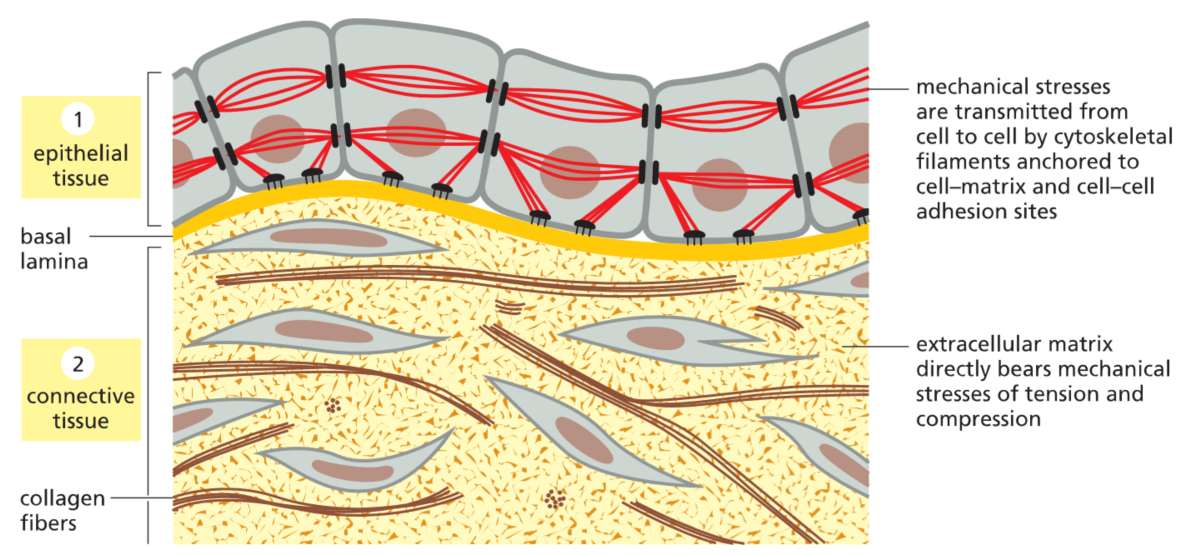
\includegraphics[width=0.7\linewidth]{tiss_overview}
	\caption{An overview of the tissue structure between the epithelial tissue and the extracelullar matrix.}
	\label{fig:tissoverview}
\end{figure}


\subsection{Cell Junctions}

There are \textbf{four main types of \gls{celljunctions}}, which each have specific functions, as well as subgroups:
\begin{enumerate}
	\item \textbf{\gls{anchoringjunctions}}: adhesion of cell-cell (c-c) or cell-matrix(c-m) connections.
	\begin{itemize}
		\item Actin related: \gls{adherensjunctions} for c-c and \gls{actinlinkedjunctions} for c-m
		\item \gls{intermediatefilamentattachmentsites}: \gls{desmosomes} for c-c and \gls{hemidesmosomes} for c-m.
	\end{itemize}
	\item \textbf{\gls{occludingjunctions}}: Block inter-cellular passage, causing impermeable or selectively permeable barriers
	\begin{itemize}
		\item \gls{tightjunctions} (vertebrates)
		\item \gls{septatejunctions} (in non-vertebrates, not covered in course)
	\end{itemize}
	\item \textbf{\gls{channelformingjunctions}}: Enable communication between two cell interiors (ex. GAP junctions - electrical conductance between two cells).
	\begin{itemize}
		\item \gls{Gapjunctions} (animals)
		\item \gls{plasmodesmata} (plants, not covered in course)
	\end{itemize}
	\item \textbf{\gls{signalrelayingjunctions}}: To enable communication between two adjacent cells (ex. neurological synapse).
	\begin{itemize}
		\item \gls{chemicalsynapses} (nervous system)
		\item \gls{immunologicalsynapses} (immune system, not covered in course)
		\item \gls{transmembraneligandreceptorcellcellsignalingcontacts} (Delta-Notch, ephrin-Eph, etc.) 
		\item Anchoring, occluding, and channel-forming junctions can all have signaling functions in addition to their structural roles.
	\end{itemize}
\end{enumerate}

\begin{figure}[H]
	\centering
	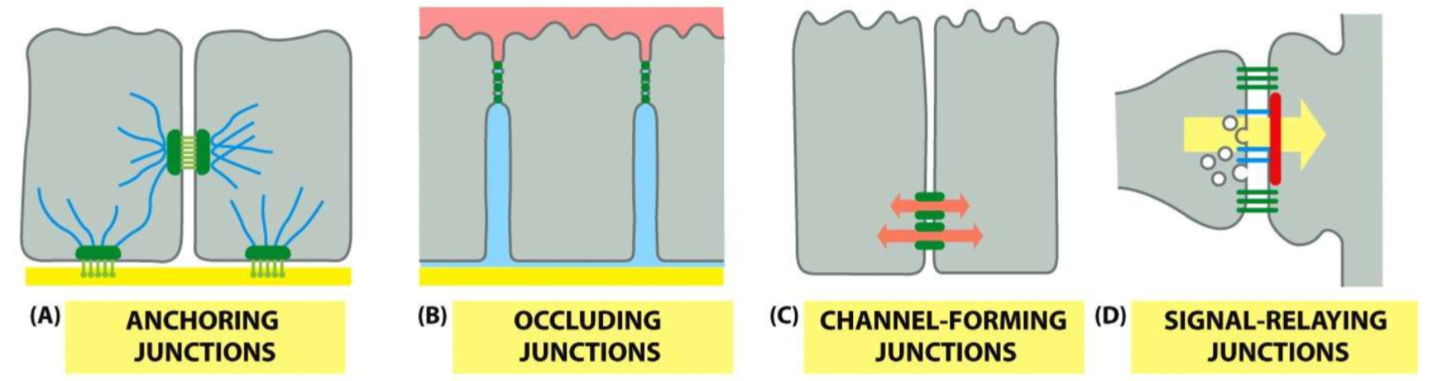
\includegraphics[width=0.7\linewidth]{junct_types}
	\caption{The four main types of junctions between cell-cell and cell-matrix.}
	\label{fig:juncttypes}
\end{figure}

The same cell will have many different types of junctions. A \textbf{\gls{junctioncomplex}} is a tight junction, at the most apical position, followed by an adheren junction, followed by a desmosome. These three "glue" a cell together. The figure \ref{fig:junctoverex} shows all the different types of junctions, based off of an epithelial cell of the small intestine: 

\begin{figure}[H]
	\centering
	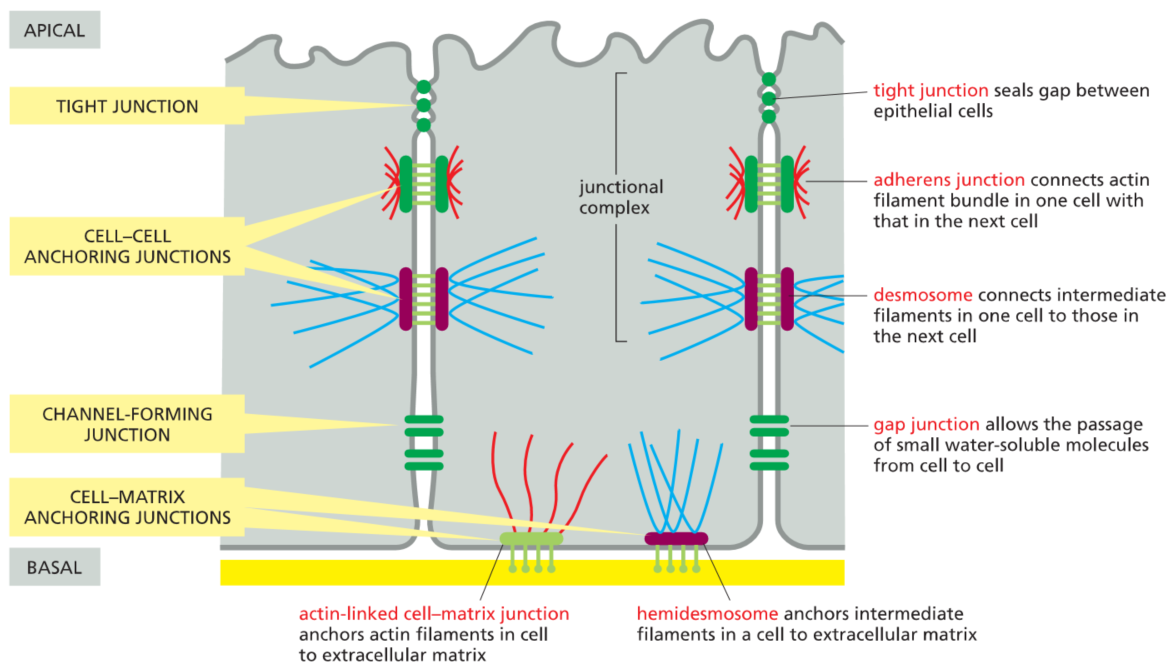
\includegraphics[width=0.7\linewidth]{junct_overex}
	\caption{An example of the types of junctions, based off of an epithelial cell in the small intestine.}
	\label{fig:junctoverex}
\end{figure}


There are two types cells bind to each other:
\begin{enumerate}
	\item \textbf{\textbf{\gls{homophilicbinding}}}: both cells have identical extracellular proteins which bind together.
	\item \textbf{\textbf{\gls{heterophilicbinding}}}: two different proteins attach to each other. Common for signaling (e.g., Delta-Notch).
\end{enumerate}

\subsubsection{Cell-Cell Anchoring Junctions}

There are four main different anchoring junctions, two for cell-cell and two for cell-matrix. Here is an overview (fig: \ref{fig:anchover}) of each type and what there main actors are:

\begin{figure}[H]
	\centering
	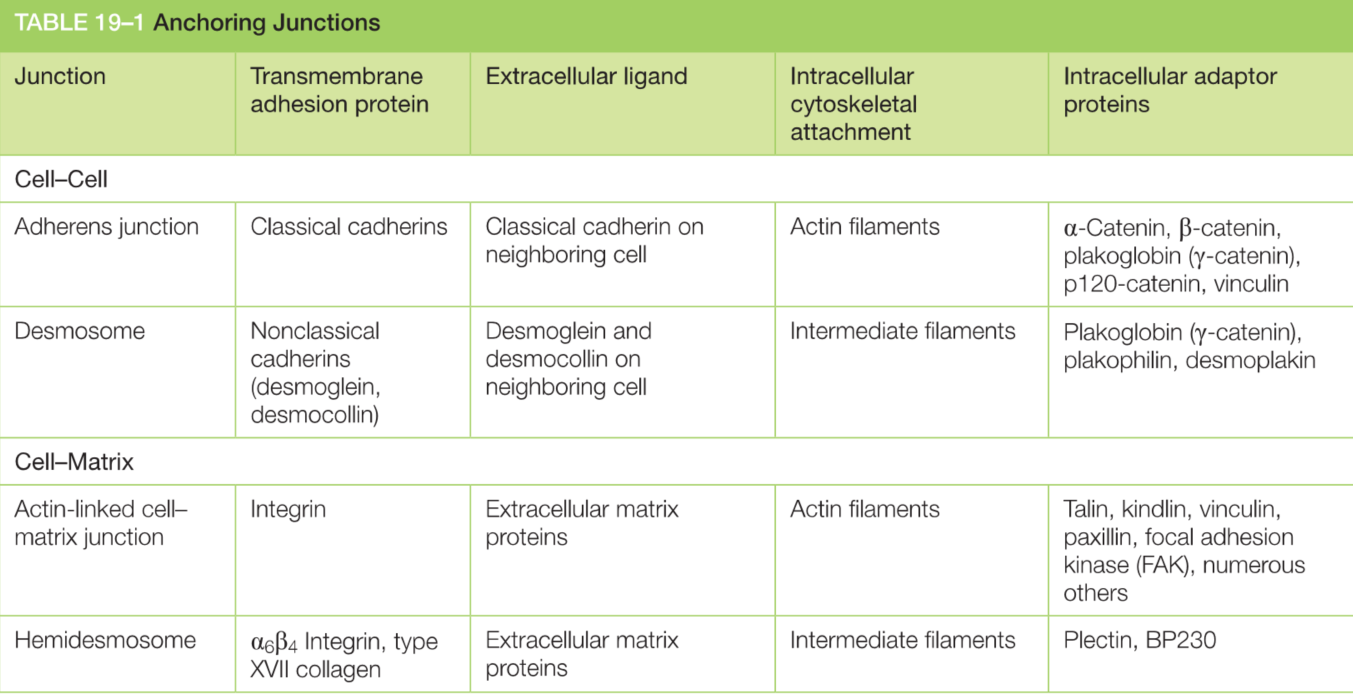
\includegraphics[width=0.7\linewidth]{anch_over}
	\caption{An overview of the different types of anchoring junctions.}
	\label{fig:anchover}
\end{figure}


\paragraph{Cadherins and Adherens Junction}

There are a lot of different \gls{cadherin} superfamily members. All of them are structurally related in the ecm domain, as they all have the cadherin domains. The number of \gls{cadherindomain} varies strongly (5 for classical, 4 or 5 for \gls{desmogleins} and \gls{desmocollins}, and at time over 30 for \gls{nonclassicalcadherins}. In addition, their functions, and intracelullar proteins vary strongly. Some even lack the transmembrane element (e.g., T-cadherin who is attached through a GPI anchor). All this means a strong variety of cadherins in the superfamily. Here (fig: \ref{fig:cadsuper}) are some examples: 
\begin{figure}[H]
	\centering
	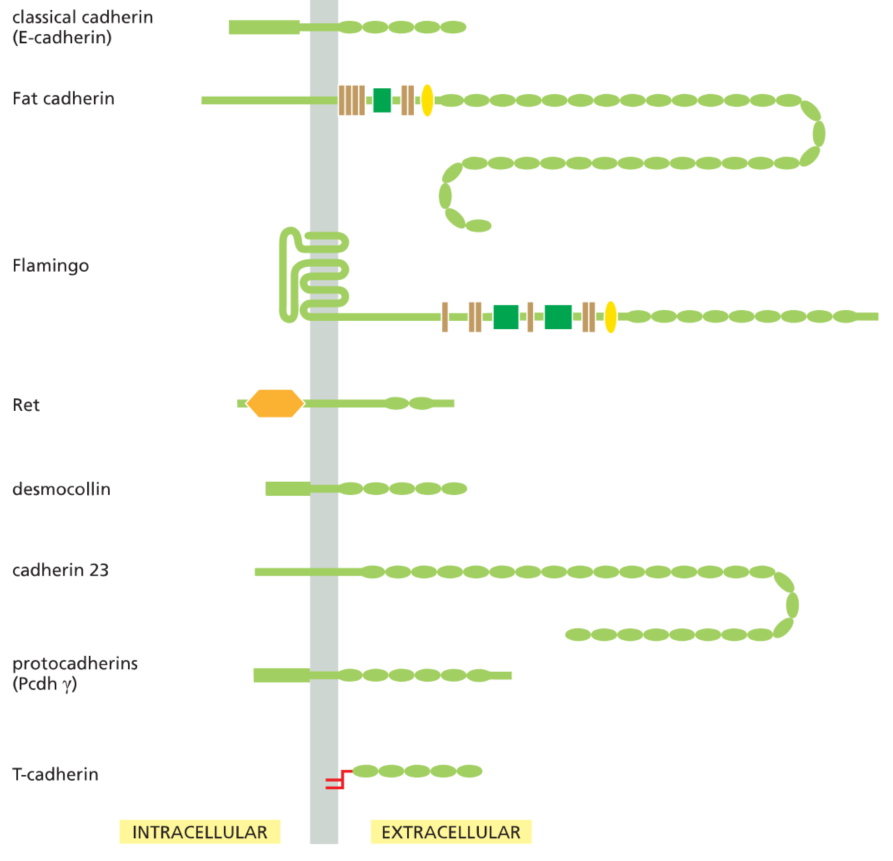
\includegraphics[width=0.3\linewidth]{cad_super}
	\caption{Shows some members of cadherin superfamily.}
	\label{fig:cadsuper}
\end{figure}

Cadherins mostly bind \textbf{homophically}. The extracellular of a classical cadherin contain five copies of the cadherin domain, separated by five flexible hinge regions. 

(see fig: \ref{fig:cadCaInt}) \gls{Ca2} ions bind in the neighborhood of each hinge, preventing it from flexing. As a result cadherin forms a rigid, curved structure, which allows it to enter in binding with another rigid cadherin. In the absence of Ca2+ the cadherin will be more flexible resulting in a floppy molecule that can't interact with a different cadherin. Leading to a failure of adhesion. This means that a \textbf{sufficiently high concentration of Ca2+ is essential for cell adhesion}.

(see fig: \ref{fig:cadnter}) To generate the cell-cell adhesion the cadherin domain at the N-terminal tip of one cadherin binds to the domain of the other cadherin.

(see fig: \ref{fig:cadCaInt}) At a typical cell junction, an organized array of cadherin molecules functions like Velcro. Cadherins on the same cell are thought to be coupled by side-to-side interactions between their N-terminals, resulting in a linear array. Each cadherin (green) will bind to a cadherin on the other cell (blue) that is in a perpedicular array to it. This will lead to a tight-knit structure.

\begin{figure}[H]
	\centering
	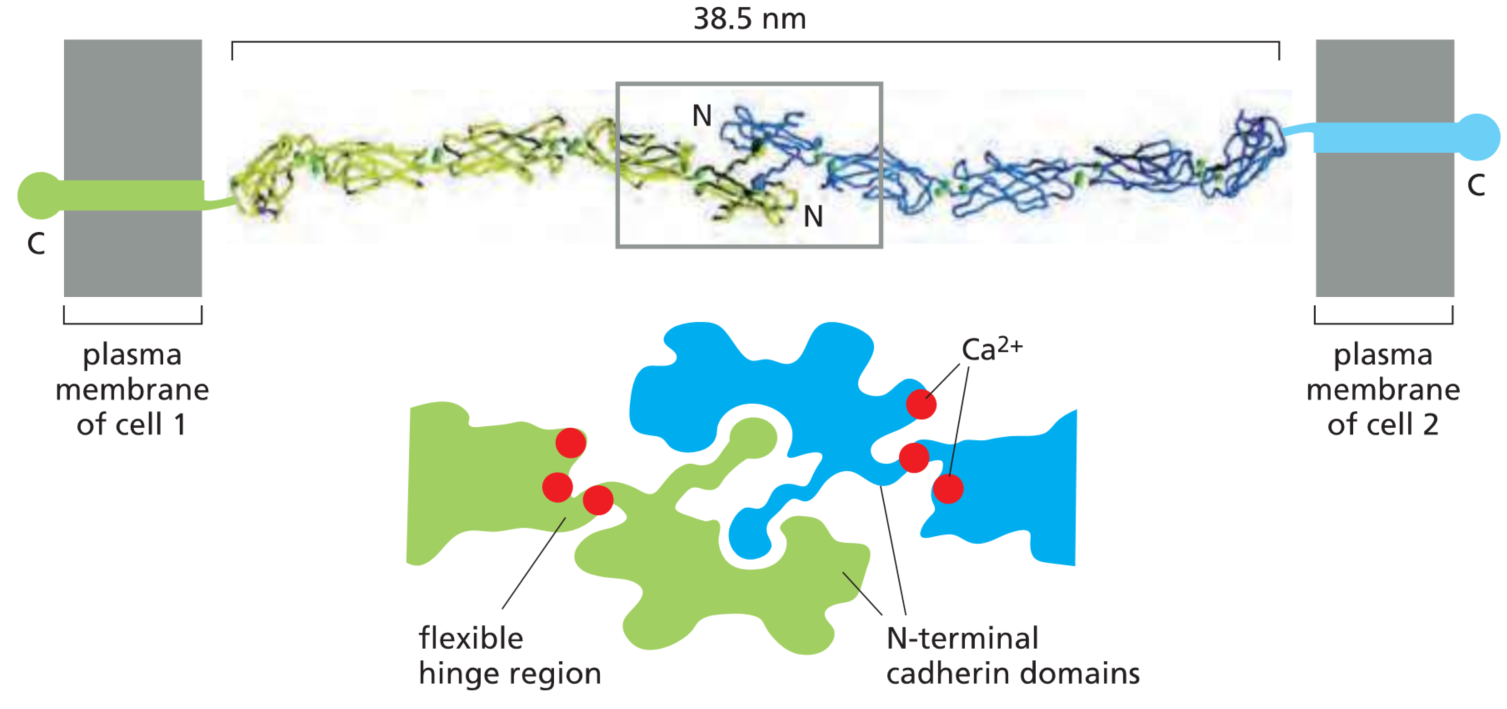
\includegraphics[width=0.6\linewidth]{cad_nter}
	\caption{The interaction between two different cadherins at their N-terminals}
	\label{fig:cadnter}
\end{figure}
\begin{figure}[H]
	\centering
	\subfigure[The interaction between cadherins and Ca2 and how it relates to stiffness of the molecule.]{
		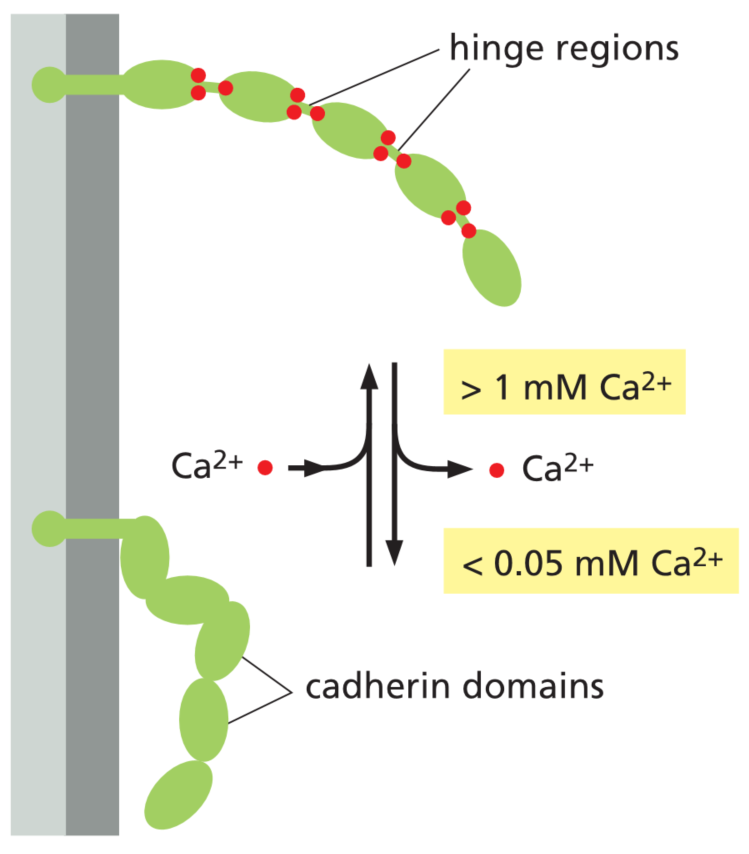
\includegraphics[width=0.4\linewidth]{cad_Ca2}
	}
	\hfill
	\subfigure[How the cadherins chain together like velcro in multiple directions. The arrays of interaction are perpendicular to each other. Having multiple arrays, then gives us a tight knit mat.]{
		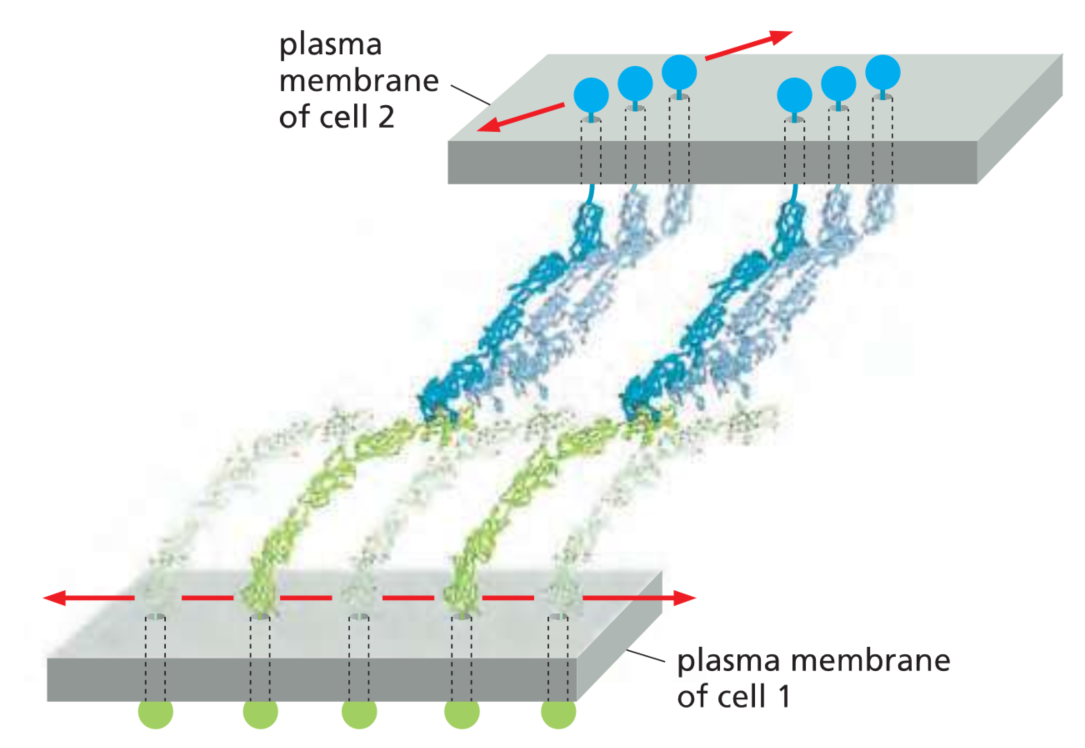
\includegraphics[width=0.5\linewidth]{cad_move}
	}
	\caption{}
	\label{fig:cadCaInt}
\end{figure}

\textbf{Classical cadherins interact with the cytoskeleton}. The interaction between cadherin and the \textbf{\gls{actin}} filaments is indirect and mediated by an adaptor complex, which includes \textbf
{\gls{betacatenin}}, which we saw in Wnt signaling (two completely different functions). Further it contains \textbf{\gls{p120catenin}} and \textbf{\gls{alphacatenin}}. Further proteins such as \textbf{\gls{vinculin}} associate with $\alpha$-catenin and provide further actin links. This mean that \textbf{multiple actins will interact with one cadherin, but through different mediator proteins}. \\

The adaptor complex will undergo a conformational change when cadherin is attached to another cadherin. The tension can also be increased through a \textbf{\gls{myosinII}}. The \textbf{increased tension on cadherin, causes $\alpha$-catenin to extend}, which in turn allows proteins like vinculin to attach associate and recruit further actins, strengthening the link between cytoskeleton and the junction. In essence, the \textbf{higher the tension, the more the cell strengthens the junction}.

\begin{figure}[H]
	\centering
	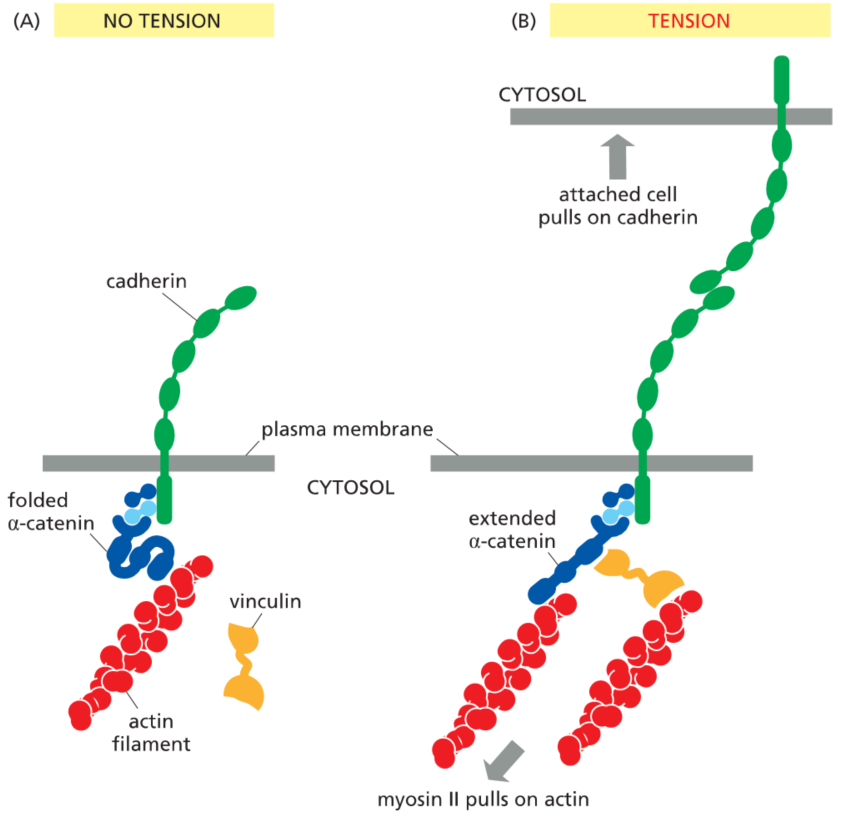
\includegraphics[width=0.4\linewidth]{cad_tens}
	\caption{How increased tension causes more recruitment of actin, strengthening the cytoskeleton and junction.}
	\label{fig:cadtens}
\end{figure}

(see fig: \ref{fig:cadexpa})This combined strengthening by cytoskeleton and junctions can organize the cells and cytoskeleton. When the first cadherin attaches it becomes easier for the neighboring ones to attach, which leads to the formation of clusters. This leads to the activation of an actin regulator, \textbf{\gls{GTPaseRac}}, which promotes further cadherin binding. This causes a more widespread junction. Eventually it is inhibited and replaced by the related \textbf{\gls{GTPaseRho}}, which moves the actins into a more linear form and promotes myosin II recruitment. That allows contractile move along the cell membrane allows cadherins up and down stream to be activated too. This further expands the junction.

\begin{figure}[H]
	\centering
	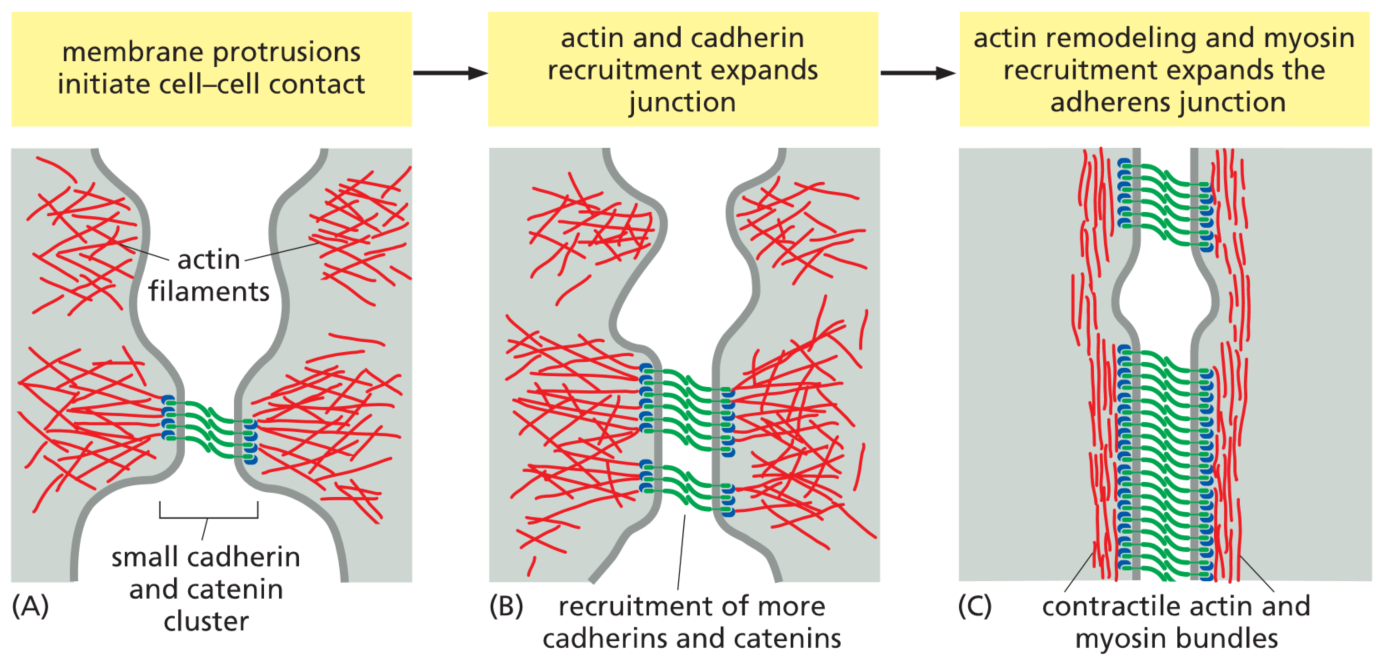
\includegraphics[width=0.6\linewidth]{cad_expa}
	\caption{The expansion of a cadherin junction.}
	\label{fig:cadexpa}
\end{figure}

\begin{RemarkWithTitel}{Sorting of cells with the help of cadherins}
	Thanks to the number of different cadherins and \textbf{homophylic nature of cadherins}, cells tend to associate better with some cell than others and sort themselves accordingly. In an experiment this was shown, by purposefully mixing up cells and then seeing them re-associate.
	
	\begin{figure}[H]
		\centering
		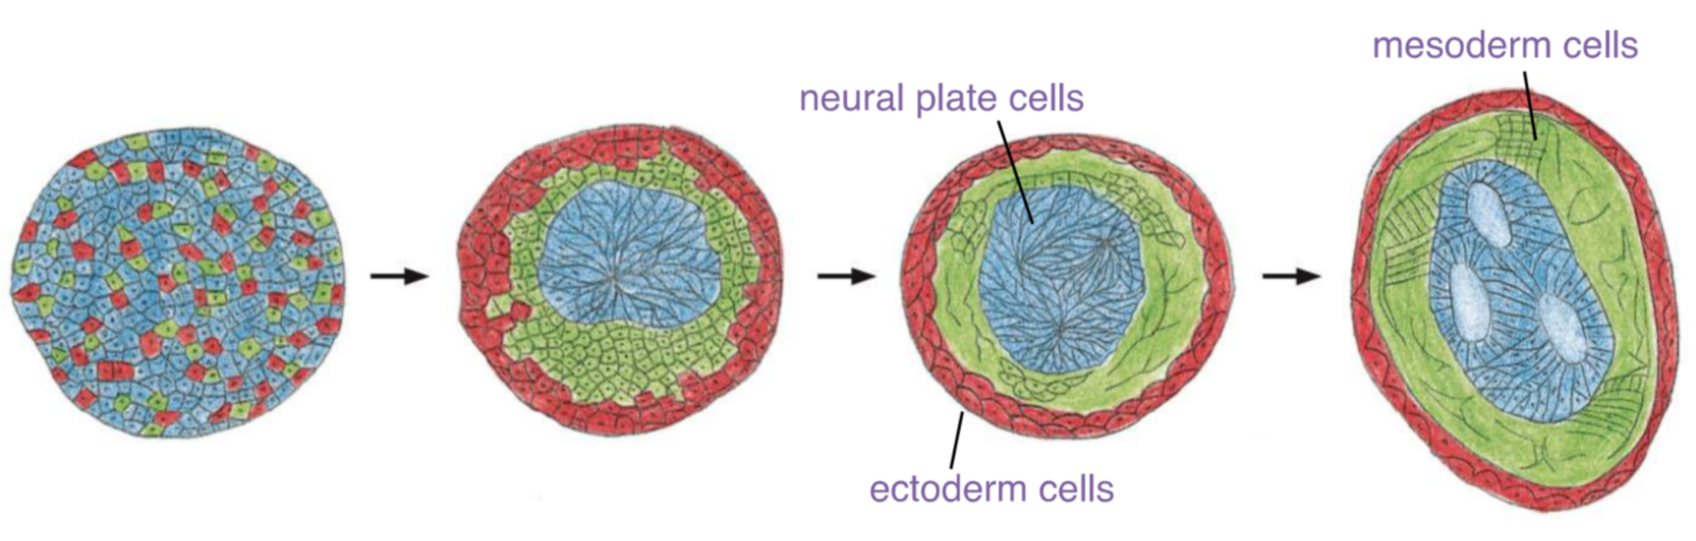
\includegraphics[width=0.5\linewidth]{cad_reas}
		\caption{This experiment shows how \textbf{cells reassociate thanks to having specific cadherin bonds}. This allows cells to sort themselves to the correct cell types.}
		\label{fig:cadreas}
	\end{figure}
	
\end{RemarkWithTitel}

\paragraph{Adhesion Belts by Adherens Junctions}

The actins in the cell between two cadherins can form a direct line from one adherens junction to one on the other side of the cell. If this line is continued between a number of cells, it forms an \textbf{\gls{adhesionbelt}}. This gives a lot of stability and allows for the formation of pretty set structures between epithelial cells. 

% error for glossary entry when compiling alone here
%uncomment the glossary entry
\begin{figure}[H]
	\centering
	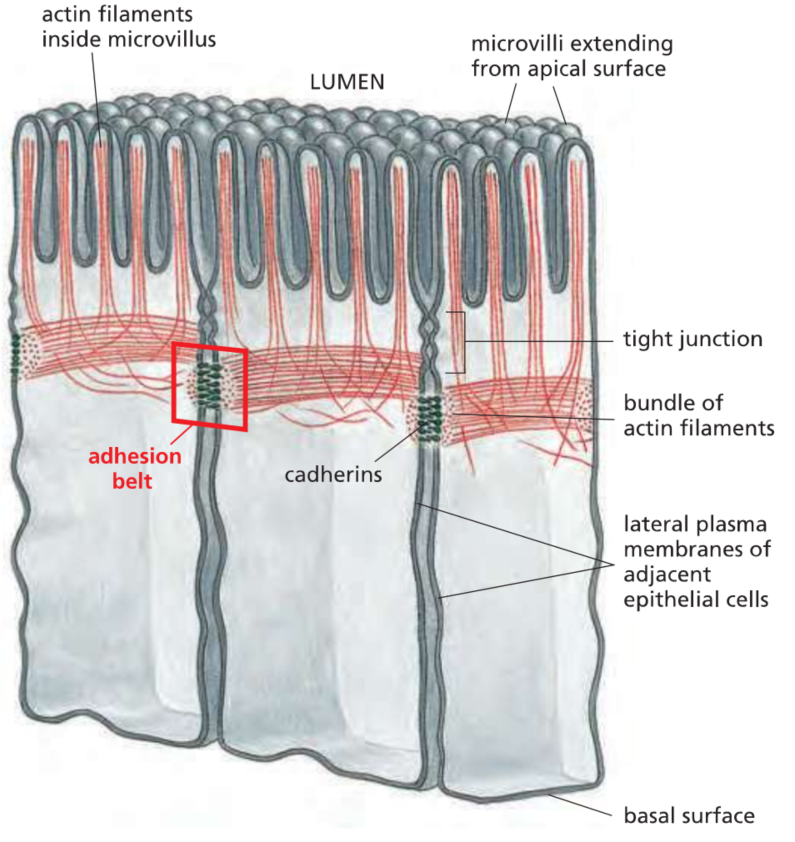
\includegraphics[width=0.4\linewidth]{cad_micr}
	\caption{Shows an example of an adhesion belt, in the case of \gls{microvilli}.}
	\label{fig:cadmicr}
\end{figure}

\begin{RemarkWithTitel}{Microvilli in the small intestine:}
	In the small intestine it is important that all the microvilli are tightly packed to maximize surface are. Adhesion belts, keep the cells in place.
\end{RemarkWithTitel}

\begin{RemarkWithTitel}{Use Case: Developmental Biology}
	The adhesion belt helps in cell development, by providing structure and connectivity between cell. For example, when creating an the neural tube in early vertebrate development, it helps the cells to narrow at their apex and roll into a tube.
	
	\begin{figure}[H]
		\centering
		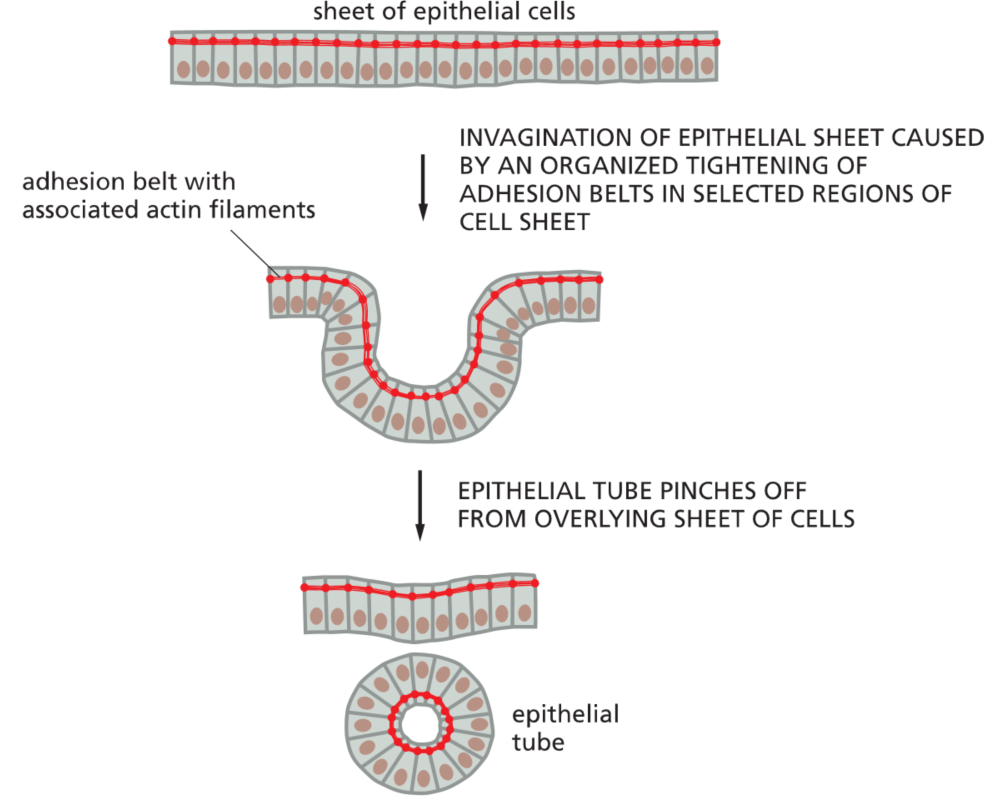
\includegraphics[width=0.4\linewidth]{cad_deve}
		\caption{How adhesions belts assist the development of cell groups.}
		\label{fig:caddeve}
	\end{figure}
	
	Looking more at the development of the neural tube, we can also observe that \textbf{at different parts of the adhesion belt, we will have different cadherins.} This will have the effect that they will segregate to each other, making it easier to break away form the \gls{ectoderm}.
	
	\begin{figure}[H]
		\centering
		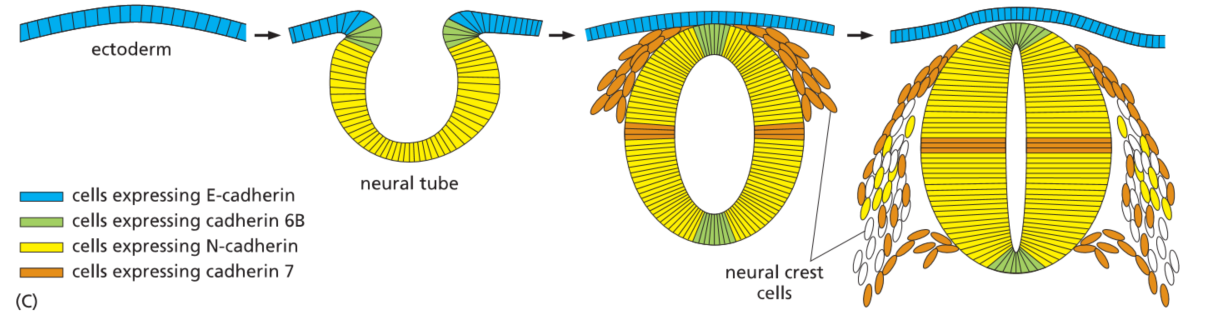
\includegraphics[width=0.7\linewidth]{cad_neur}
		\caption{How having different cadherins causes certain shapes to form, looking at the use case of neural development.}
		\label{fig:cadneur}
	\end{figure}
	
\end{RemarkWithTitel}

\paragraph{EMT and MET}

Some key terms and their meaning:
\begin{itemize}
	\item \gls{mesenchymal}: multipotent stromal (connective tissue) cells that differentiate into a variety of cells including: fibroblasts, osteoblasts, chondrocytes, adipocytes, myocytes.
	\item \gls{EMT}: epithelial-to-mesenchymal transition
	\item \gls{MET}: Mesenchymal-to-epithelial transition
\end{itemize}

Now, looking at the \textbf{EMT} first: epithelial cells loose their polarity, as well as their cell adhesion, through the dissolution of tight junctions, adherence junctions (with that E-cadherin and cytoskeletal reorganization), and desmosomes. \\

Next up \textbf{MET}:  starting with the initial adhesive contact, then the adherens junction (with it cytoskeletal reorganization), and then the desmosome associateion. Finally tight junctions will form.

\begin{figure}[H]
	\centering
	\subfigure[Shows the cycle of met and emt epithelial and mesenchymal cells can go through.]{
		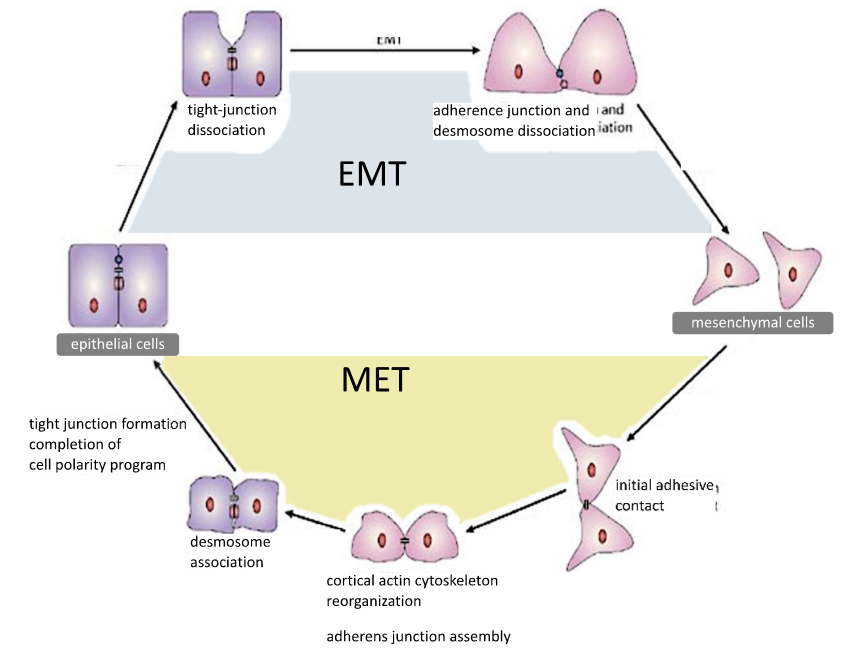
\includegraphics[width=0.5\linewidth]{met_emt}
		}
		\subfigure[Shows how cancer uses EMT and MET]{
		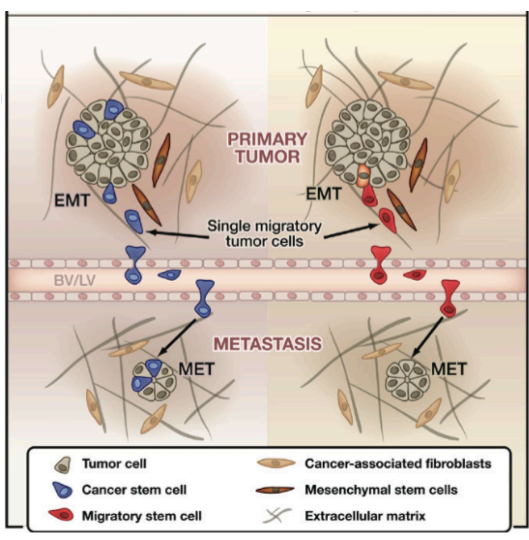
\includegraphics[width=0.4\linewidth]{met_canc}
	}
	\caption{}
	\label{fig:metemt}
\end{figure}

\begin{RemarkWithTitel}{The body applying EMT and MET}
	\textbf{EMT} is used in:
	\begin{itemize}
		\item \textbf{embryonic development}: helps cell move, adapt to for new cell gorups;
		\item \textbf{Wound healing}: helps cells migrate to wound;
		\item \textbf{Cancer metastasis}: allows cells to migrate.
	\end{itemize}
	\textbf{MET} is used in:
	\begin{itemize}
		\item \textbf{embryonic development}: helps tissue grow together, form, and specialize (less talked about);
		\item \textbf{Wound healing}: crucial in repair of damage (fills the gaps);
		\item \textbf{Cancer metastasis}: allows it to settle into new area.
	\end{itemize}
\end{RemarkWithTitel}

\begin{RemarkWithTitel}{Some transcription factors which regulate EMT}
	\textbf{\gls{Twist}, \gls{Snail}, \gls{Slug}, and \gls{Zeb}} are transcription factors that \textbf{drive EMT}. They do this by repressing epithelial genes (mainly cadherins) or activating mesenchymal genes (\gls{fibronectin} and \gls{vimentin}).
\end{RemarkWithTitel}

\paragraph{Desmosomes and Hemidesmosomes}
\label{sec:demso}

The structure of a desmosome is as follows:
\begin{itemize}
	\item On the cytoplasmic surface is a \textbf{dense plaque composed of a mix of intracellular adaptor proteins}. Some of these components are:
	\begin{itemize}
		\item \textit{\gls{desmogleins}} and \textit{\gls{desmocollins}} are \gls{nonclassicalcadherins}. Their tails bind to \textit{\gls{plakiglobin}} ($\gamma$-catenin) amd \textit{plakophillin} (distant relative of p120-catenin). Together they turn into a \textit{desmoplakin}.
		\item \textbf{Desmoplakin} binds to the sides of intermediate filaments, tying the \gls{desmosomes} to the filaments.
	\end{itemize}
	\item To this plaque a bunch of keratin \textbf{intermediate filaments} are attached.
	\item On the other side of the plaque a lot of \textbf{\gls{nonclassicalcadherins}} bind to the plaque, whose extracellular domains interact with the \gls{cadherin} of another molecule.
\end{itemize}

\begin{figure}[H]
	\centering
	\subfigure[Shows a rough overview of how a desmosome anchor junction looks like.]{
		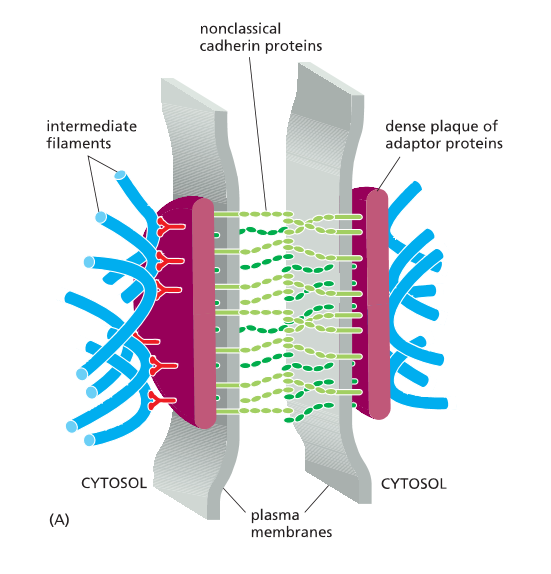
\includegraphics[width=0.4\linewidth]{desm_over}
	}
	\subfigure[Shows the plaque in more detail.]{
		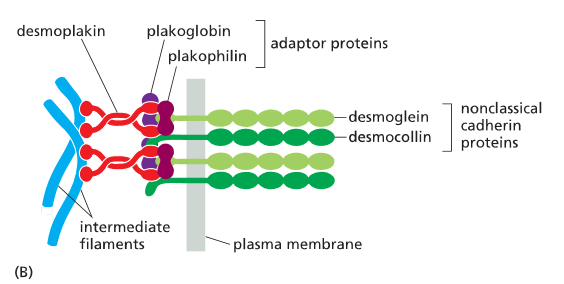
\includegraphics[width=0.55\linewidth]{desmo_dets}
	}
	\caption{}
	\label{fig:desm}
\end{figure}

While a \textbf{desmosome is cell-cell a hemidesomosome is cell-matrix} (hence hemi = half). For the cell side of things the structure is exactly the same. Both types of junctions give rigidity to the cell.

\subsubsection{Tight Junctions}

\gls{tightjunctions} are everywhere, like tracts in the urinary system. 

Tight junctions \textbf{hold adjacent membranes very close together}. The strands are composed of transmembrane proteins that make contact across the intercellular space, creating a seal. They due this multiple times in high numbers, which creates a very large surface area and with that a strong seal. The sealing strand is composed mainly of proteins with four transmembrane elements. The main one is \textbf{\gls{claudin}}, secondary \textbf{\gls{occludin}} have less of an important role in determining \textbf{junction permeability}. The two termini for both this proteins are on the cytoplasmic side of the membrane where they interact with scaffolding proteins and link to actin to organize the sealing strands.

\begin{figure}[H]
	\centering
	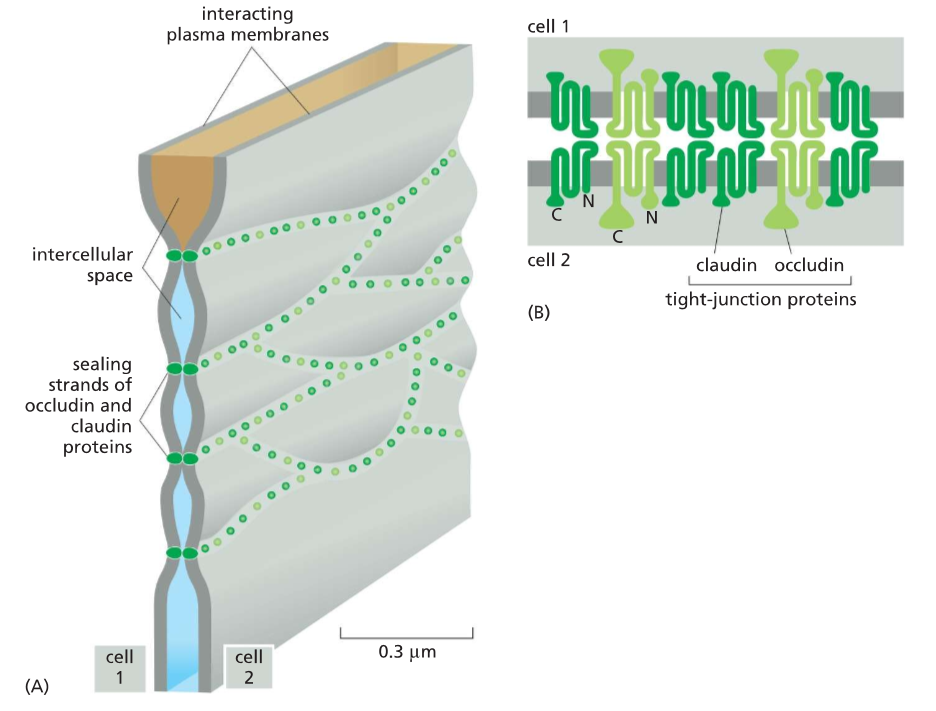
\includegraphics[width=0.6\linewidth]{tight_over}
	\caption{Shows a model of a tight junction. Highlights how sealing strands exist around the molecule. Also shows the main two sealing proteins: claudin and occludin.}
	\label{fig:tightover}
\end{figure}


\begin{RemarkWithTitel}{3D-thinking of tight junctions}
	In 3D these tight junctions will wrap around the cell forming a band. As otherwise they wouldn't actually block anything if they just existed at selected spots
\end{RemarkWithTitel}

\subparagraph{Tight Junctions in transcellular transport: Intestine}

Tight junctions \textbf{seal off different parts of the tissue}. This allows for the body to create transfers from one part to the other in a more controlled version. Tight junctions also confine transport proteins to their part of the membrane, working as a \textbf{fence}, within the lipid bilayer. They also \textbf{block the backflow} of unwanted molecules.

\begin{figure}[H]
	\centering
	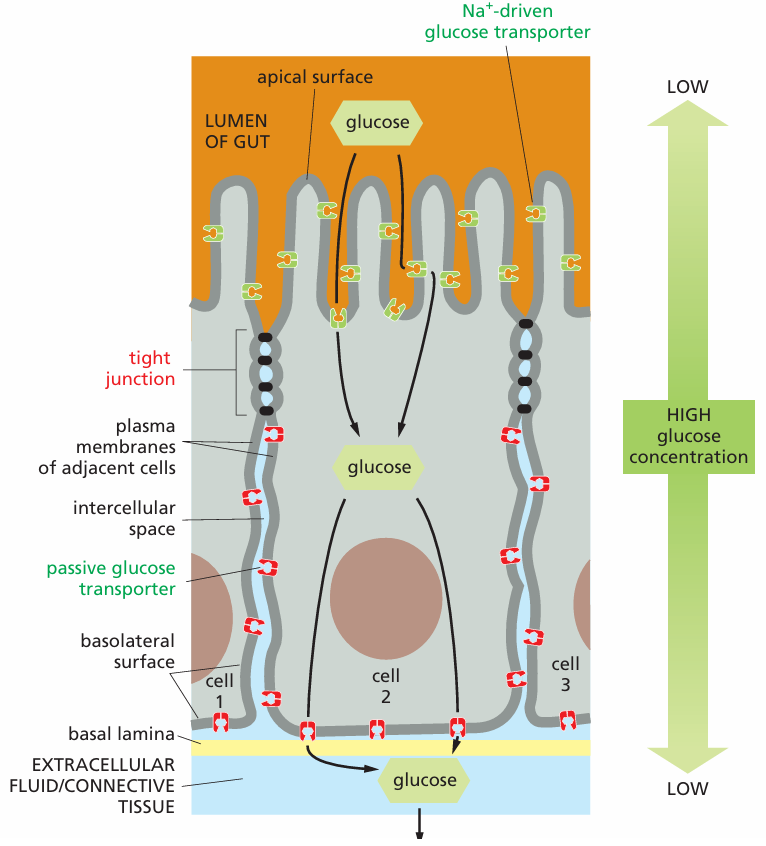
\includegraphics[width=0.6\linewidth]{tight_glu}
	\caption{Shows the intake of glucose in the small intestinge. For simplicity only tight junctions are shown of the anchor junctions. Glucose is actively transported into the cell through Na+-driven glucose transporters and leaves passively through glucose transporters.}
	\label{fig:tightglu}
\end{figure}


\subsubsection{Channel-Forming Junctions}

The essence: \textbf{Gap junctions decide which molecules are shared between cells}. However, there is a limit at around \textbf{1000 Daltons}.

The gap junction is seen as a cluster of homogeneous intramembrane particles. Each intramembrane particle is a protein assembly called a \textbf{\gls{connexon}}, consisting of \textbf{6 \gls{connexin} subunits}, which penetrate the lipid bilayer. Connecting two connexons then creates a channel between two cells. These connexons can be \textbf{\gls{homotypic}} or \textbf{\gls{heterotypic}}, depending on the usage of different conenxins. Each connexin consists mainly of $\alpha$-helix, with the whole connexon ending up having a pore size of around 1.4nm which matches with the molecule size permitted (around 1000 Daltons).

\begin{figure}[H]
	\centering
	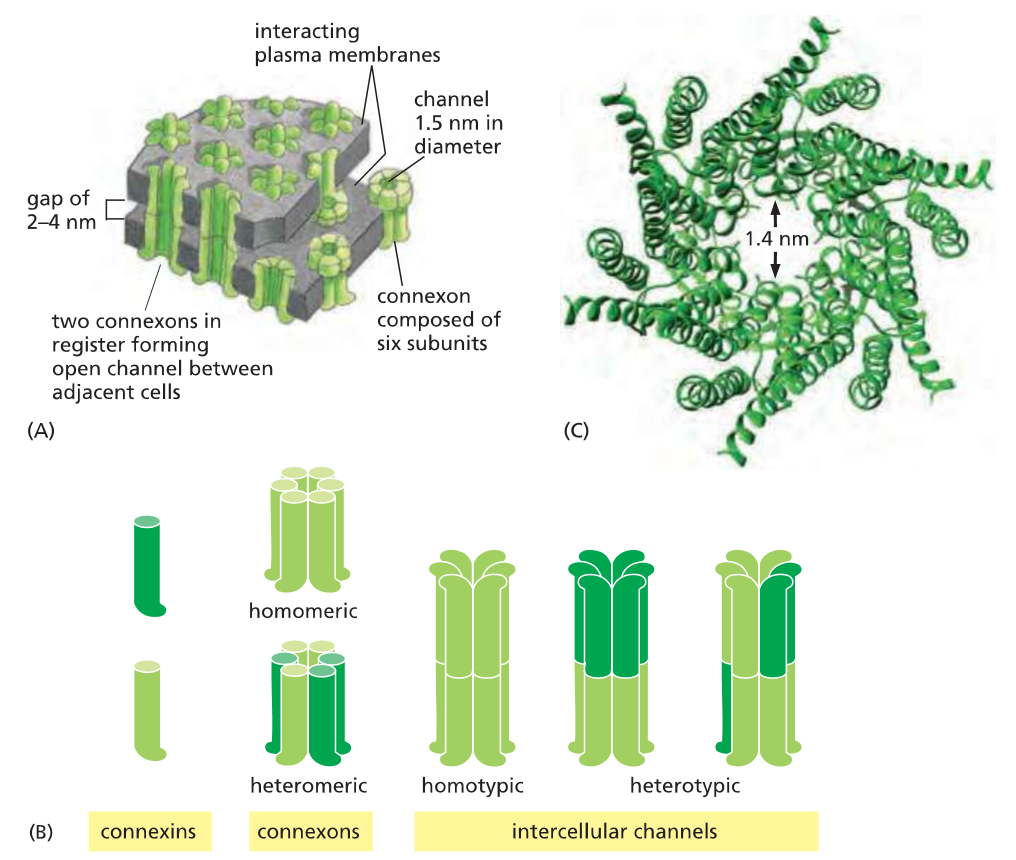
\includegraphics[width=0.8\linewidth]{gap_over}
	\caption{(A) Shows the view on the membrane, (B) the components of a connexon, (C) and the 3D structure of a connexon.}
	\label{fig:gapover}
\end{figure}


\subsection{The Extracellular Matrix}

The extracellular matrix (ECM) is a complex, \textbf{dynamic scaffold that provides structural support to tissues, regulates cell behavior, and helps organize cells into functional assemblies}.\\
The major components of the extracellular matrix are the following:

\begin{itemize}
	\item \gls{glycoprotein}: \gls{laminin}, \gls{nidogen}, and \gls{fibronectin}  
	\\ \textit{Analogy: Like \textbf{connectors and adaptors} in a mechanical system, these proteins bind various ECM elements and cell receptors, \textbf{organizing the matrix} and enabling communication between the cell and its surroundings.}
	
	\item \gls{fibrous}: \gls{typeIVcollagen}, \gls{fibrillarcollagen}  
	\\ \textit{Analogy: These act like scaffolding beams, providing \textbf{tensile strength and structural integrity to tissues}. Type IV collagen forms meshworks in the basal lamina, while fibrillar collagens (e.g., type I, II, III) form rope-like fibers in connective tissue.}
	
	\item \gls{proteoglycan} and \gls{glycosaminoglycanGAGs}: \gls{hyaluronan}, \gls{perlecan}, \gls{decorin}, \gls{aggrecan}  
	\\ \textit{Analogy: These are like sponges, \textbf{highly hydrated} and act like \textbf{space-filling molecules that resist compression}, and serve as reservoirs for signaling molecules.}
\end{itemize}

\begin{figure}[H]
	\centering
	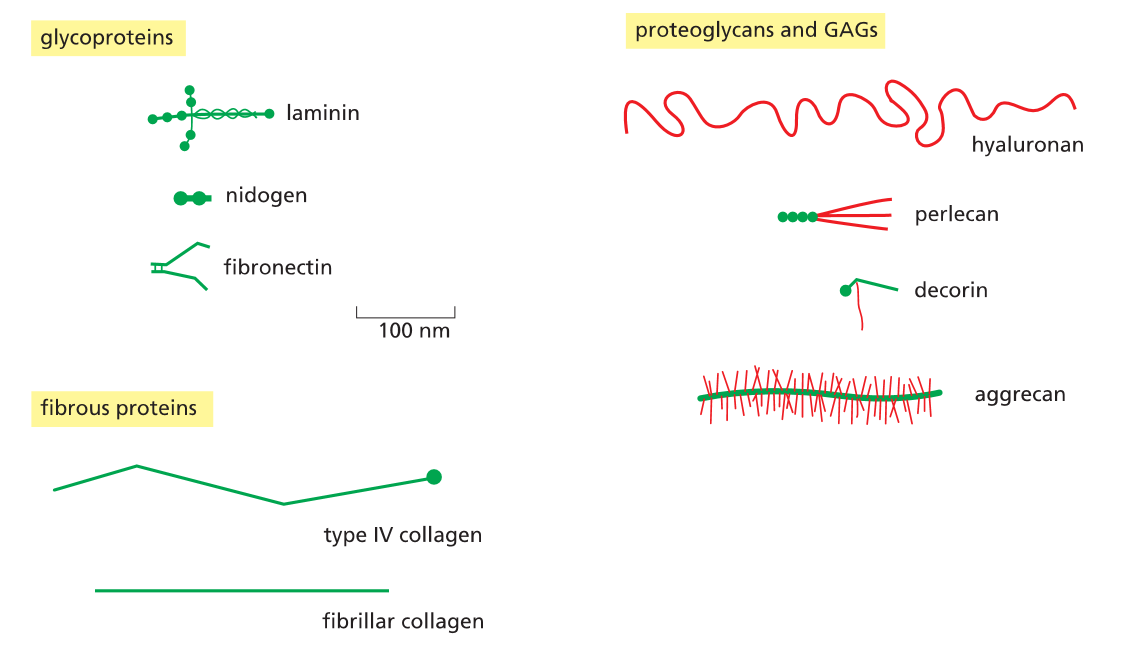
\includegraphics[width=0.6\linewidth]{ecm_comp}
	\caption{Shows the major components of the ecm. Green is protein and red is GAG.}
	\label{fig:ecmcomp}
\end{figure}

The size of these molecules also varies very much:
\begin{itemize}
	\item globular protein (MW 50'000)
	\item glycogen (MW around 400'000)
	\item spectrin (MW 460'000)
	\item collagen (MW 290'000)
	\item hyaluronan (MW 8 x $10^{6}$ and 300nm in diameter)
\end{itemize}

\subsubsection{Proteoglycan and GAGs}
Proteoglycan and GAGs form structures like sponges in the ECM, and act like space-filling molecules that resist compression.\\
GAGs are a long chain of \textbf{typically sulfated repeating disaccharides}, this means that we will need a bunch of glycosylation bonds. Something about \textbf{GAGs is that they are often sulfated}. Thus they are highly \textbf{negative charged}. It will vary from 70\% (\gls{heparin}) to under 50\% (heparan) or none at all (\gls{hyaluronan}). Further the length can vary from 200 pairs of disaccharides to up to 25'000 sugar monomers, again highlighting the high variability. Moreover, the disaccharide chain is also very variable: for \textbf{\gls{chondroitinsulfate}} it is D-glucuronic acid and N-acetyl-D-galactosamine, while for \textbf{\gls{heparansulfate}} it is N-acetyl-D-glucosamine with either D-glucuronic acid or L-iduronic acid, and finally for \textbf{\gls{keratansulfate}} it is D-galactose and N-actyl-D-glucosamine. 

\begin{figure}[H]
	\centering
	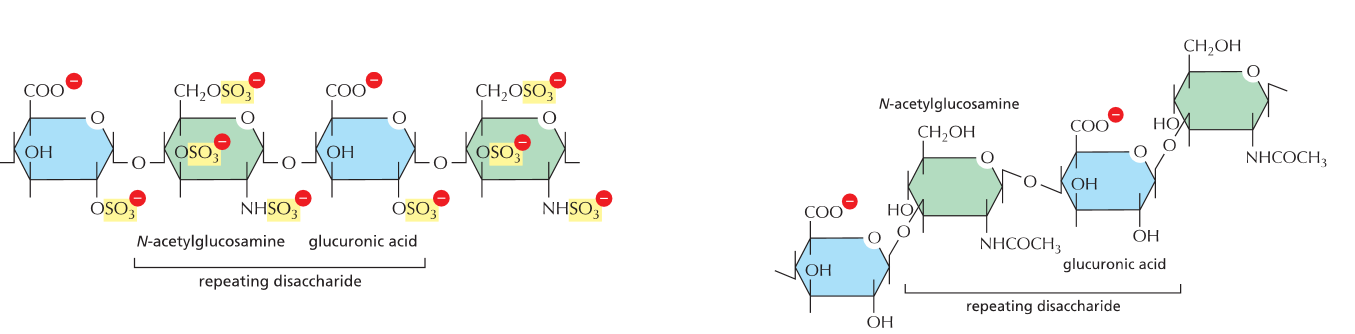
\includegraphics[width=0.8\linewidth]{gag_sulf}
	\caption{The picture on the left shows a GAG with 100\% sulfation (not really a thing). On the right we can see hyaluronan, a rather simple but long GAG (no sulfation).}
	\label{fig:gagsulf}
\end{figure}
 

\subparagraph{Synthesis proteoglycan: adding GAGs to proteins}

GAGs are added to their core protein via a special link tetrasaccharide of the GAG and a serine on the protein. Once this linkage has happened the rest of the GAG repeating disaccharide chain can be added one sugar at a time. 

\begin{figure}[H]
	\centering
	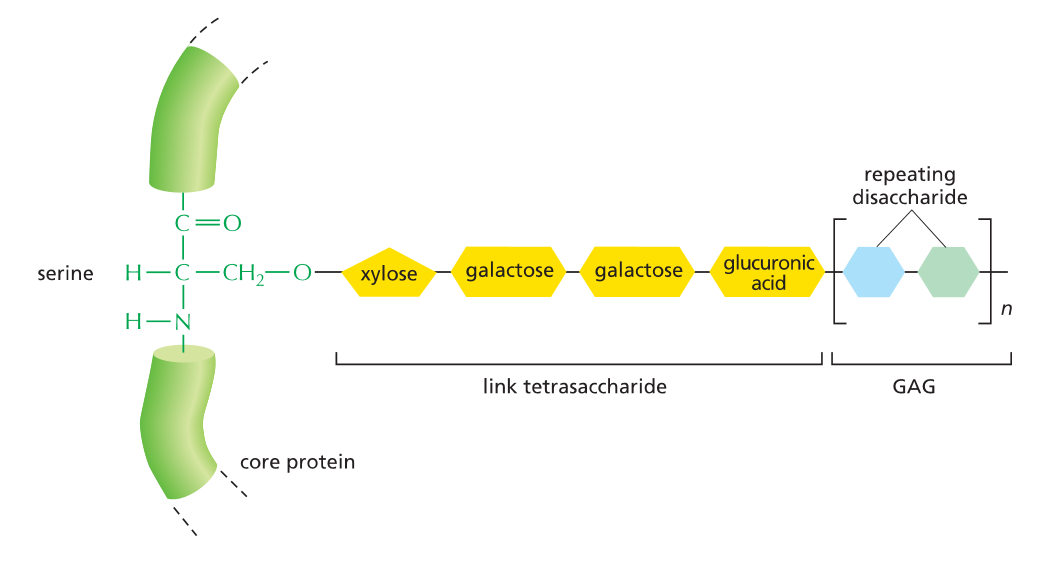
\includegraphics[width=0.7\linewidth]{gag_bond}
	\caption{How a proteoglycan bind the GAG and protein.}
	\label{fig:gagbond}
\end{figure}

\begin{RemarkWithTitel}{Proteoglycans varies a lot}
	The Glycosylation degree is very variable in size and absolute number. Aggrecan for example has 300 amino acids in its core protein and 30 keratan sulfate and 100 chondroitin sulfate chains linked to the protein. On the other hand decorin just has one GAG and "decorates" collagen fibrils (so it can't be all too large).
	
	\begin{figure}[H]
		\centering
		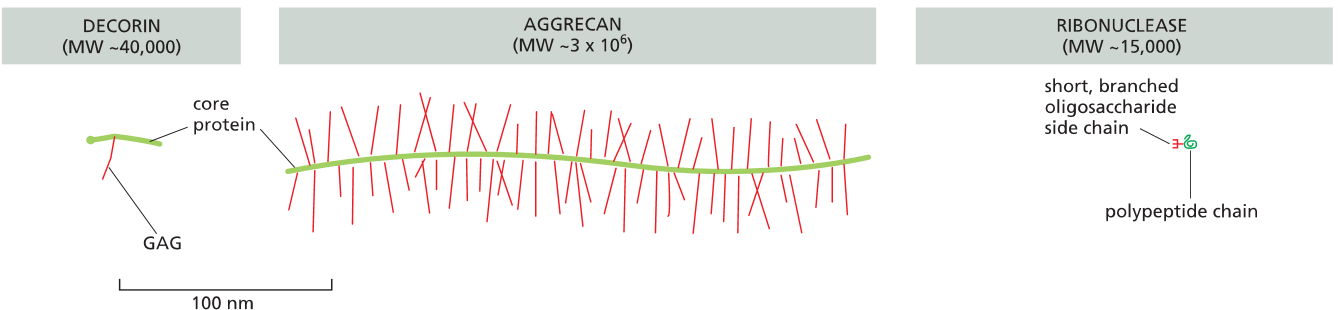
\includegraphics[width=0.7\linewidth]{gag_ex}
		\caption{Different proteoglycans and their varying sizes and numebrs of glycosylations.}
		\label{fig:gagex}
	\end{figure}
	
\end{RemarkWithTitel}

\paragraph{Aggrecan aggregation}

Aggrecan is a \textbf{proteoglycan}. It has many keratan sulfate glycosylations. The N-terminal of aggrecan then \textbf{binds noncovalently to a single hyaluronan} molecule (not a proteoglycan itself, it is a GAG but very special one). A link protein, part of the hyaluronan-binding proteins (can also be cell surface proteins), then binds to both the aggrecan core and the hyaluronan stabilizing the bond. This \textbf{gel-like aggregate} can become huge north of $10^{8}$ daltons and occupy the volume of a bacterium (2x$10^{-12}cm^{3}$).

\begin{figure}[H]
	\centering
	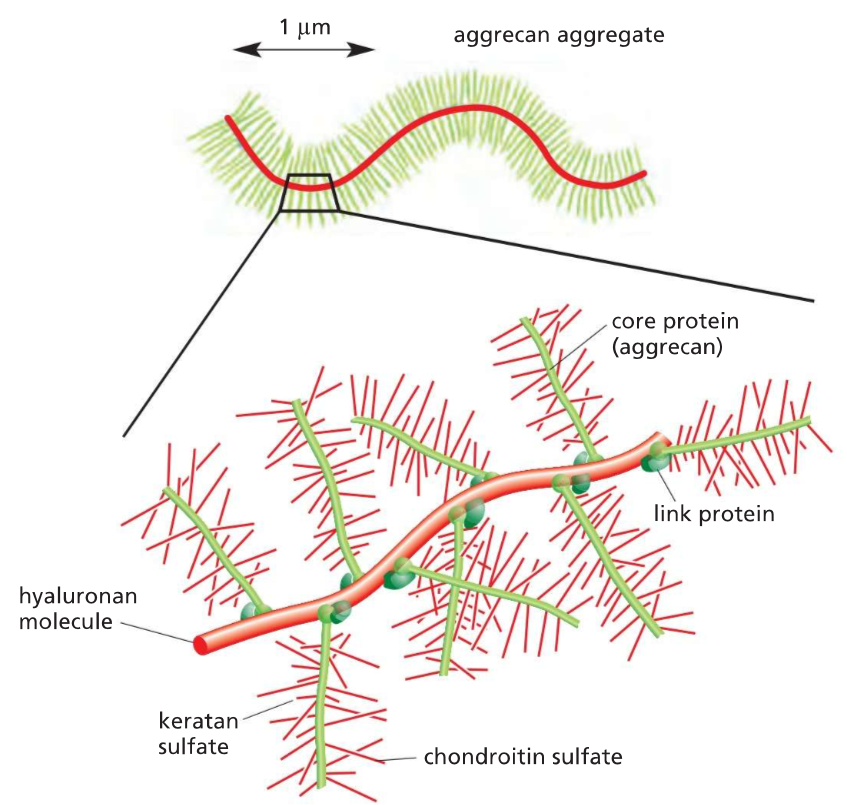
\includegraphics[width=0.5\linewidth]{agg_comp}
	\caption{A visualization of the aggrecan aggregate on a hyaluronan molecule}
	\label{fig:aggcomp}
\end{figure}

\subsubsection{Collagen}
Collagen act like scaffolding beams in the ECM, providing tensile strength and structural integrity to tissues.
\subparagraph{Structure of a typical collagen}
Collagen is composed of three $\alpha$ chains. One $\alpha$ chain is a long left-handed helix with a set pattern: \textbf{every third amino acid is a \gls{glycine}}. The reason being, for the three $\alpha$ chains to wrap into each other, one of the amino acids needs to fit in between and the only amino acid small enough for that is glycine. The entire collage will become up to 300nm long.\\
\indent The other two can be anything but are commonly a \gls{hydroxyproline} (Y) (modified during collagen synthesis) or a \gls{proline} (X).The \textbf{hydroxylation reactions are \textbf{\gls{VitaminC}} dependent}, as it is a cofactor for the \textbf{enzymes \gls{lysylhydroxylase} and \gls{prolylhydroxylase}}. \textit{Scurvy, vitamin C deficiency}\\
The hydroxylation is important to stabilize the triple helix, enable cross-linking, and ensure proper function and secretion.

\begin{figure}[H]
	\centering
	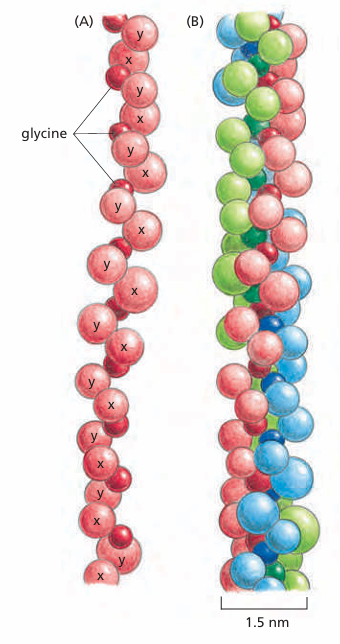
\includegraphics[width=0.3\linewidth]{coll_struc}
	\caption{Structure of collagens. X is typically proline and y hydroxypriline}
	\label{fig:collstruc}
\end{figure}

\begin{RemarkWithTitel}{Collagen as connective Tissue: Fibrils}
	\gls{collagenfibers} are organized into bundles which run through the ECM. They are oriented in nearly a right angle, creating a net of fibrils. 
\end{RemarkWithTitel}

\subparagraph{Collagen types}
\begin{figure}[H]
	\centering
	\subfigure[A bunch of different types of collagen]{
		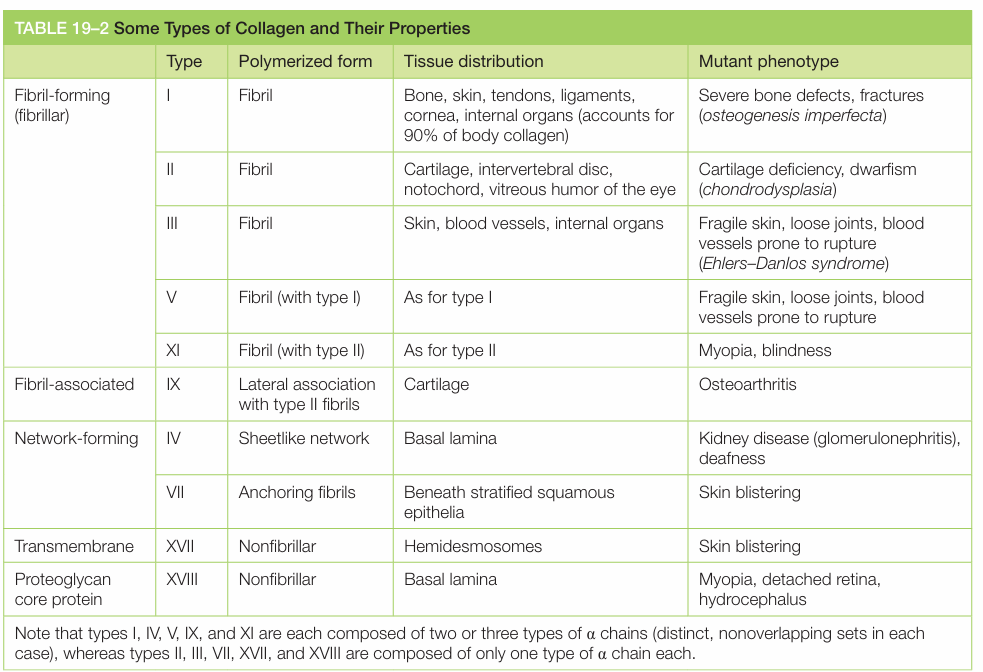
\includegraphics[width=0.5\linewidth]{coll_type}
	}
	\subfigure[(a) shows how collagen forms its trimeric form, and then from it all the diverse forms it can take.]{
		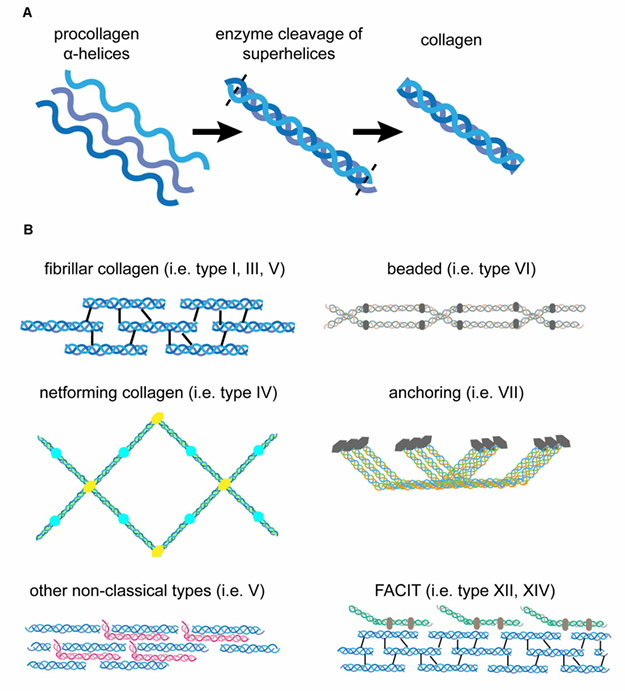
\includegraphics[width=0.4\linewidth]{coll_typeI}
	}
\end{figure}
\textbf{Fibrillar collagens} (like types I, III, and V) form rigid fibers that make the \textbf{ECM strong and stiff}. In contrast, collagen \textbf{IV forms a flexible}, network-like structure typical of the \textbf{basal lamina}, resulting in a much softer ECM.

\subparagraph{Synthesis of fibril Collagen I}

The synthesis of \textbf{\gls{collagenI}} happens in \textbf{\gls{fibroblasts}}. It happens in three parts: first \gls{procollagen} is assembled in the ER, then in the cytosol the fibril is assembled. The fiber is then assembled in the ECM. Breaking down the individual parts: \\

\textbf{Procollagen assembly}
\begin{enumerate}
	\item \textbf{\gls{procollagen}} assist folding into the left handed $\alpha$-helix
	\item \textbf{\gls{hydroxylation}} of Proline and Lysine
	\item N-linked glycosylation
	\item Beginning of quaterny structure through self-assembly of disulfide bonds.
	\item Proline bonds are also forced to be trans so they don't break apart the helical form.
	\item Formation of the triple helix
	\item transportation through \textbf{\gls{Golgiapparatus}}
	\item Modification of N- and O- linked sugars \\
	
	\textbf{Fibril/fiber assembly}
	\item Cleavage of \textbf{\gls{propeptides}}, which are the parts of the chain which didn't form the tight triple helix
	\item Self assembly of fibril
	\item Secretion
	\item Fiber assembly
\end{enumerate}

\begin{figure}[H]
	\centering
	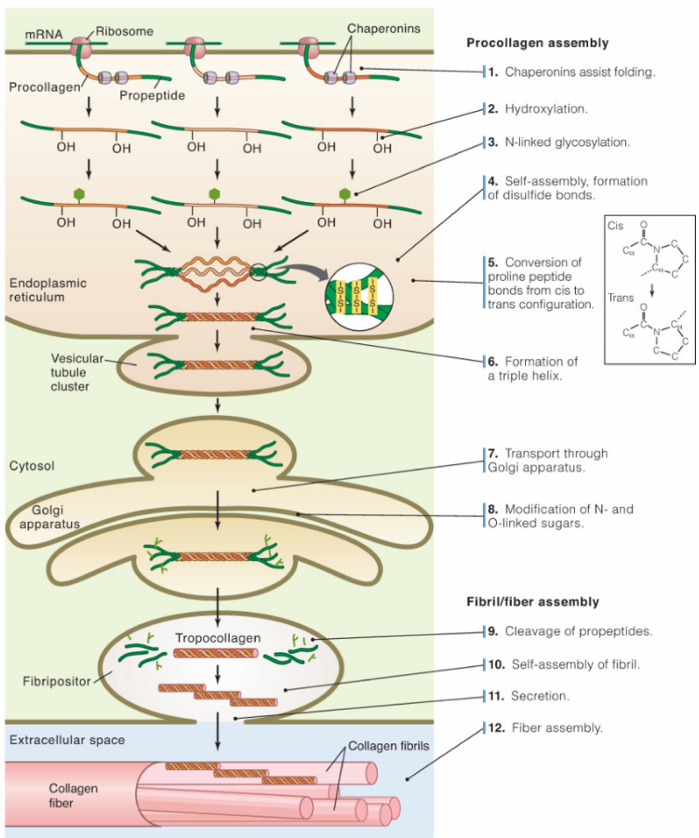
\includegraphics[width=0.6\linewidth]{coll_synt}
	\caption{Synthesis of Collagen I a type of fibril.}
	\label{fig:collsynt}
\end{figure}


\subparagraph{Defective collagen synthesis = bad news}

Having a defect in one of the proteins can be really bad really fast, as for the fibril fibers to do their job, we need everything to be packed very tightly in just the right way. For example a mutation in the gene for the \textbf{\gls{procollagenNproteinase}}, which is responsible for cutting the the parts of the gene which didn't fold properly. This will basically just mean that the collagen becomes useless.

\begin{figure}[H]
	\centering
	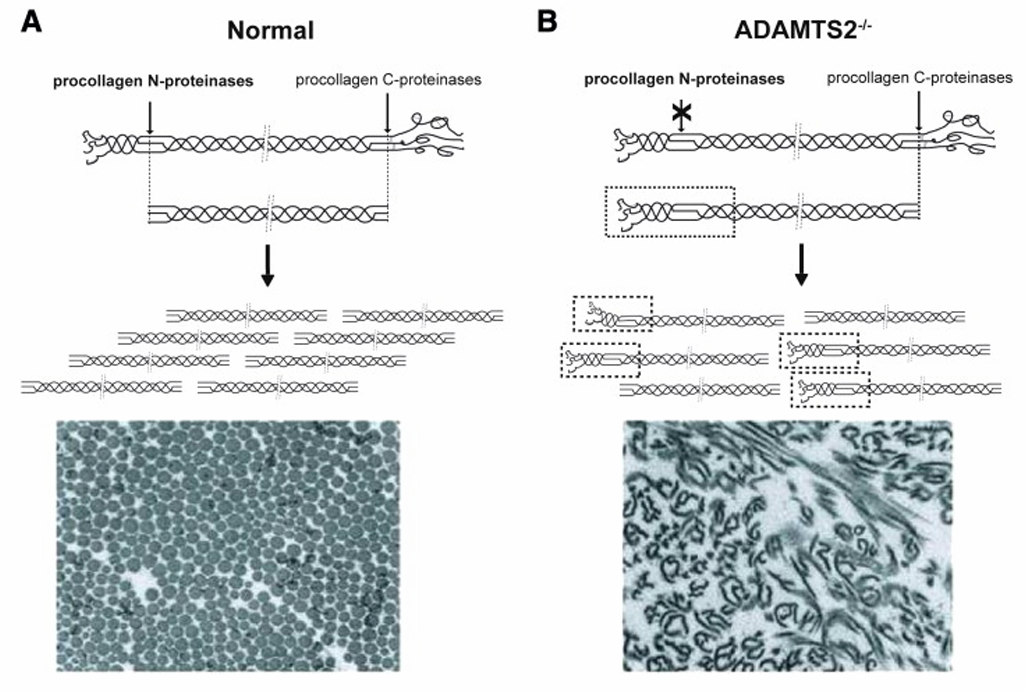
\includegraphics[width=0.6\linewidth]{coll_defe}
	\caption{How a defect in collagen synthesis is very very bad.}
	\label{fig:colldefe}
\end{figure}


\paragraph{The ECM's Flexibility}

Unlike soccer (a.k.a. football) players the ecm needs to be able to stretch. For this it has a \textbf{\gls{elastin} fiber}. It is a bunch of elastin molecules bonded covalently to generate a cross-linked network. Each molecule can extend and coil, which allows the fiber as a whole to function as a rubber band. One elastin has a \textbf{long half life of around 40 years}. However, elastin is \textbf{not really regenerated after puberty}, which lead to Gesichtsfalten. 

\begin{figure}[H]
	\centering
	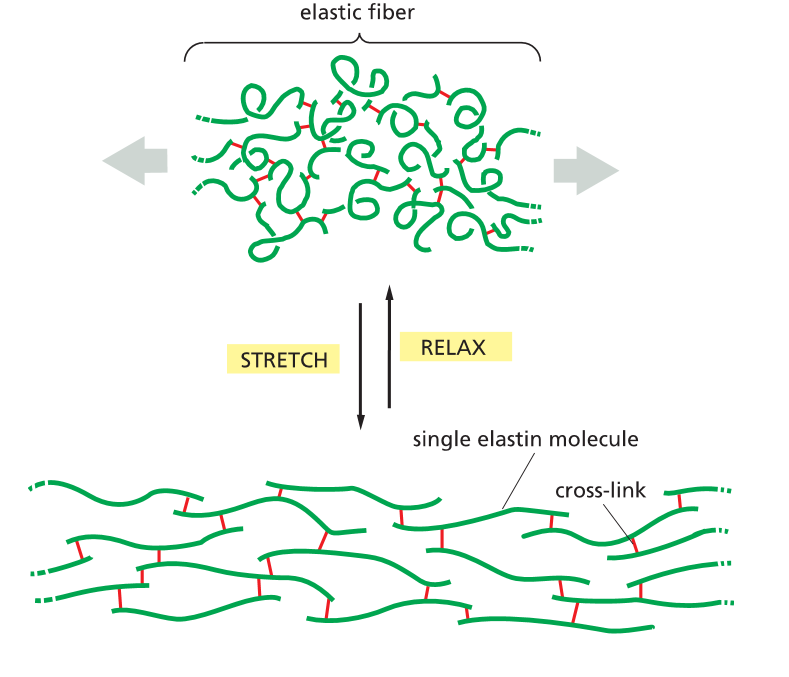
\includegraphics[width=0.5\linewidth]{ela_over}
	\caption{Elastin in its stretched vs. relaxed state.}
	\label{fig:elaover}
\end{figure}

\subsubsection{Complex Glycoproteins}
Glycoproteins perform critical roles in cell–ECM interactions, they are like connectors or organizers.\\
There are over 200 matrix glycoproteins in mammals. Many matrix glycoproteins are large \gls{scaffoldproteins} containing multiple copies of specific protein-interaction domains. Each domain is folded into a discrete globular structure, often having a bead like structure. Each protein contains multiple repeat domains. 
Example of \textbf{Fibronectin} which has a numerous copies of different \gls{fibronectin} repeats: \gls{FN1}, \gls{FN2}, and \gls{FN3}. Two type III at the end are crucial for integrin binding, while other position are important fibrin, collagen, or heparin binding.\\
\\ 
Other matrix proteins contain \textbf{\gls{EGFepidermalgrowthfactor}} (epidermal growth factor) like sequences, indicating that they might serve a similar signaling purpose. Others on the glycoprotein, like the \gls{IGFBPInsulingrowthbindingfactor} (IGFBP) regulate soluble growth factors. Many of these genes can be spliced, leading to even more diversity among glycoproteins.

Finally some of the domains are responsible for building multimeric forms. For example in fibronectin the C-termini builds dimers, in \gls{tenacin} and \gls{thrombospondin} form N-terminally linked hexamers and trimers, respectively.

\begin{figure}[H]
	\centering
	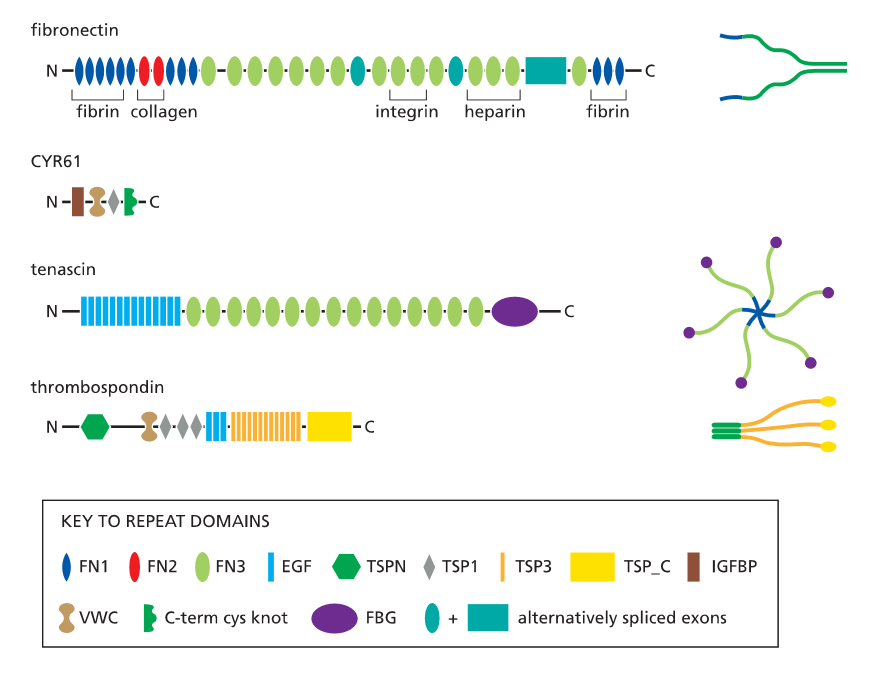
\includegraphics[width=0.6\linewidth]{glyc_comp}
	\caption{A bunch of complex glycoproteins in the ECM.}
	\label{fig:glyccomp}
\end{figure}

\paragraph{Fibronectin}
\gls{fibronectin} plays a crucial role in guiding cell structure and behaviors.

\begin{figure}[H]
	\centering
	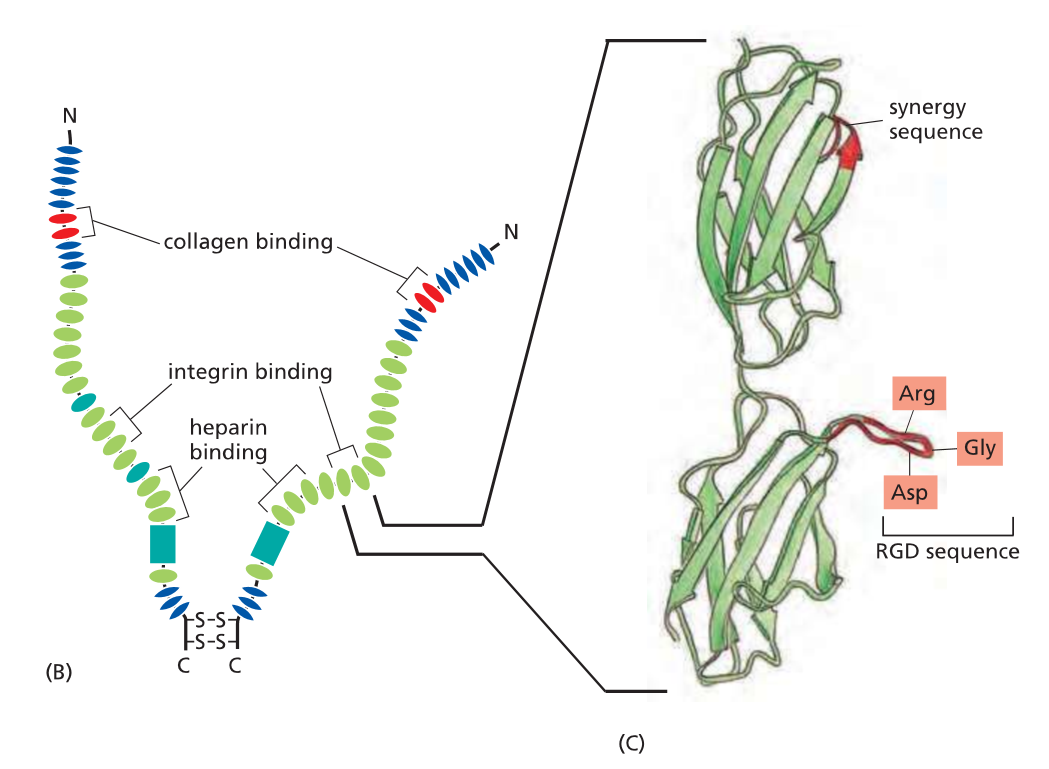
\includegraphics[width=0.6\linewidth]{fibr_struc}
	\caption{The structure of fibronectin. Note its minor differences between the chains.}
	\label{fig:fibrstruc}
\end{figure}

Looking at the fig: \ref{fig:fibrstruc} above we can see on the left that the \textbf{two chains} may be similar but not entirely the same, meaning they were spliced differently (as the same gene). They are \textbf{joined by two disulfide bonds} near the C-termini. Each chain is around 2'500 amino acids long and is folded into a bunch of domains. Some domains are specialized to binding to certain molecules. \\
The \textbf{\gls{RGD} (Arg-Gly-Asp)} is a short, conserved amino acid motif found in fibronectin and several other extracellular matrix proteins. It serves as a key \textbf{recognition site for \gls{integrin}}, enabling cells to adhere to the ECM. When integrins bind to the RGD motif, they transmit signals that regulate cell shape, movement, and survival—making RGD crucial in processes like wound healing and tissue organization.

\begin{RemarkWithTitel}{Fibronectin under tension}
	Some type III fibronectin repeats can unfold when fibronectin is put under tension. That unfolding can expose cryptic binding sites resulting in multiple in the formation of multiple fibronectins.
\end{RemarkWithTitel}

\begin{figure}
	\centering
	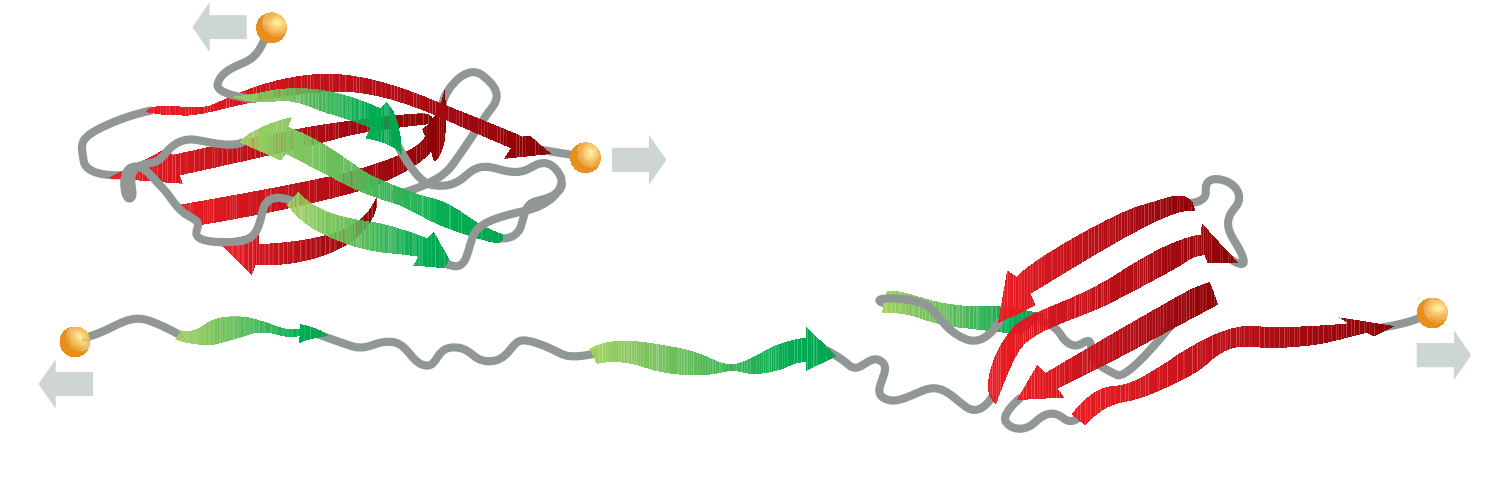
\includegraphics[width=0.4\linewidth]{fibr_tens}
	\caption{Shows how some domains are exposed when fibronectin is pulled upon.}
	\label{fig:fibrtens}
\end{figure}

\begin{RemarkWithTitel}{Fibronectins and the cytoskeleton alinging}
	Fibronectin will accumulate at focal adhesions, making the organized in a paralell way to actin filaments. Integrin molecules link the fibronectin outside the cell to the actin filaments inside it (will be covered in more detail in section \ref{integrins}). Tension on the fibronectin exposes them exposing sites which promote fibril formation.
\end{RemarkWithTitel}

\subsubsection{Basal Lamina}
The basal lamina is a specialized, \textbf{thin sheet of the extracellular matrix (ECM)} that underlies and supports epithelial cells, muscle fibers, adipocytes, and Schwann cells. Depending on where we are in the body, the basal lamina will have a\textbf{ different organization}. These differences in composition can also exist between tissues.
\begin{figure}[H]
	\centering
	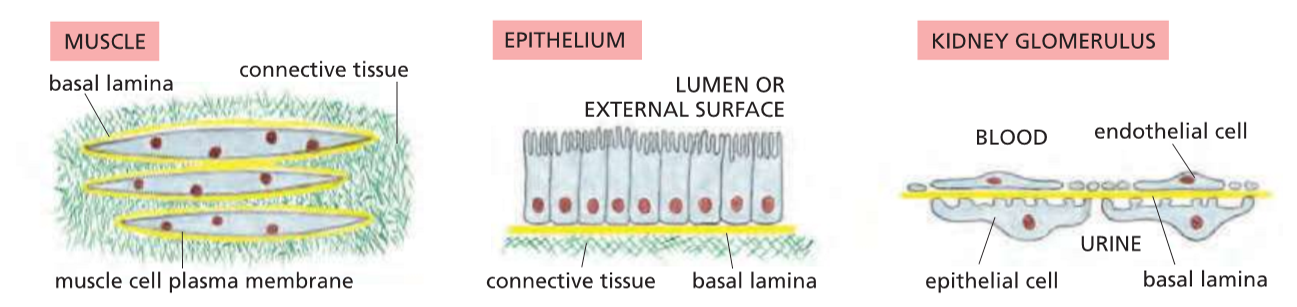
\includegraphics[width=0.7\linewidth]{bl_diff}
	\caption{The basal lamina will look very different depending on where in the body it is.}
	\label{fig:bldiff}
\end{figure}

The \gls{basallamina} is formed by specific interaction between proteins, \textbf{\gls{laminin}},\textbf{ \gls{typeIVcollagen}}, and \gls{nidogen}, and the \gls{proteoglycan} \gls{perlecan}. \textbf{Transmembrane laminin receptors}, \textbf{\gls{integrin}} and \gls{dystroglycan} are thought to organize the assembly of the basal lamina.

\begin{figure}[H]
	\centering
	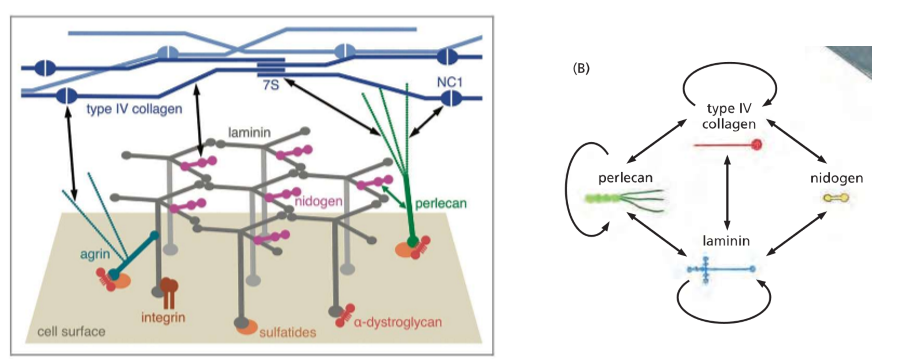
\includegraphics[width=0.8\linewidth]{bl_form}
	\caption{The assembly of the basal lamina is very complex. On the right, one can see the net of interaction. An arrow indicates who can bind to who.}
	\label{fig:blform}
\end{figure}

\subsubsection{Integrins}
\label{integrins}

Integrins  (\textit{glycoprotein}) are essential \textbf{transmembrane receptors} that mediate \textbf{cell–extracellular matrix (ECM) and cell–cell adhesion}. They connect the ECM to the intracellular cytoskeleton, allowing cells to sense and respond to their external environment. Structurally, \textbf{integrins span the plasma membrane as $\alpha$-helical domains}, anchoring them firmly in the lipid bilayer. Each integrin is a heterodimer made of an $\alpha$ and a $\beta$ subunit, and together they \textbf{bind ECM components like fibronectin, laminin, and collagen}. Upon binding, they transmit mechanical and chemical signals across the membrane, influencing cell shape, migration, survival, and gene expression.
\begin{figure}[H]
	\centering
	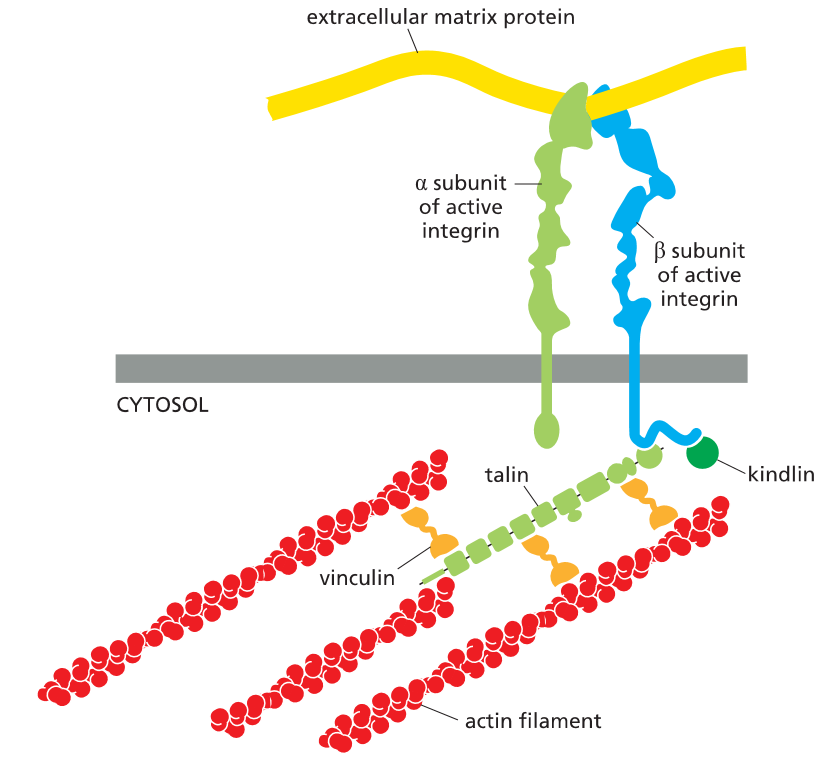
\includegraphics[width=0.4\linewidth]{int_roug}
	\caption{A rough glance at integrins role for the basal lamina}
	\label{fig:introug}
\end{figure}

\subparagraph{The types of integrins}

\begin{figure}[H]
	\centering
	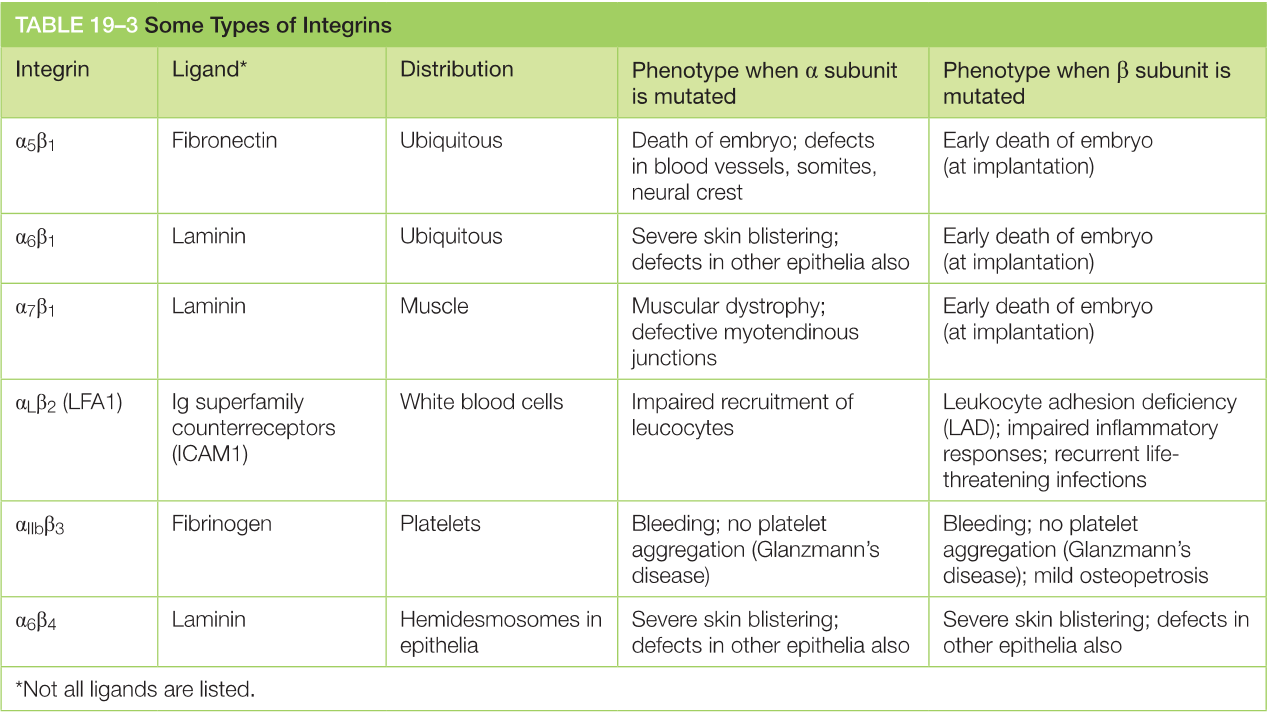
\includegraphics[width=0.6\linewidth]{int_type}
	\caption{Some types of integrins}
	\label{fig:inttype}
\end{figure}

\subparagraph{Integrin: The Major Activity States}

Integrin has to main states: inactive (folded) and active (extended). This switch happens spontaneously.
\begin{figure}[H]
	\centering
	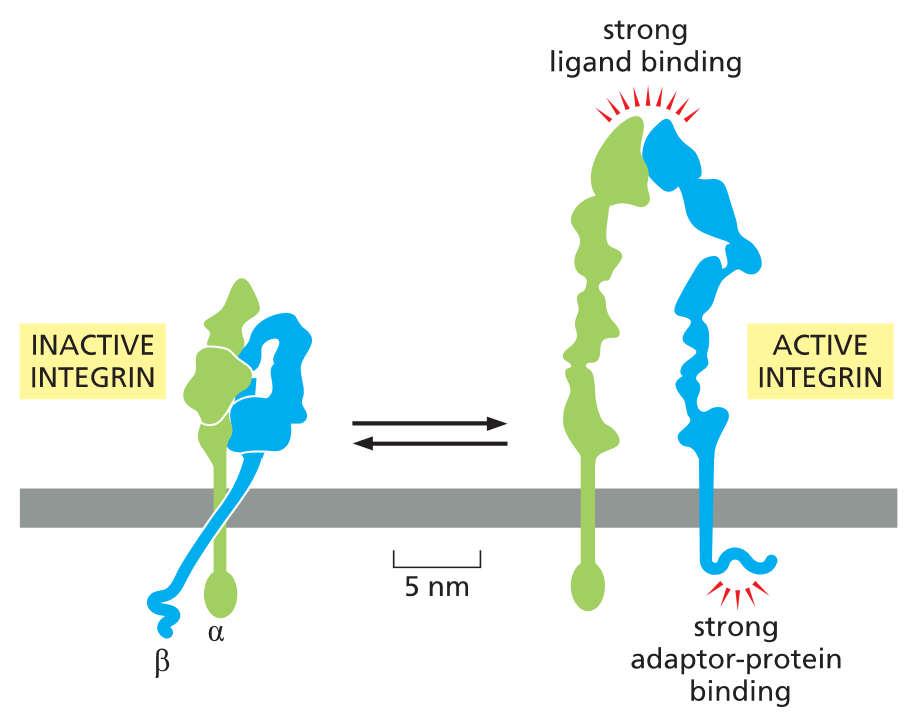
\includegraphics[width=0.6\linewidth]{int_conf}
	\caption{The two different conformations of integrins.}
	\label{fig:intconf}
\end{figure}


\subparagraph{Integrins in hemidesomoses}

Hemidesomoses (see sec:\ref{sec:desmo}) glue epithelial cells to the basal lamina. They do this by linking keratin filaments on the inside and out outside of the cell. A specialized integrin($\alpha$6, $\beta$4) attaches to the \textbf{keratin} filaments, via adaptor proteins \textbf{\gls{plectin}} and \textbf{\gls{BP230}} and to the laminin extracellularly. The adhesive complex also contain a unusual collagen known as \textbf{\gls{collagenXVII}}, which has a membrane-spanning domain attached to its extracellular collagenous portion.

\begin{RemarkWithTitel}{Blisters due ot hemisdesomoses}
	Defects in any of these proteins may cause blistering of the skin. One such disease \textbf{\gls{bullouspemphigold}} is an autoimmune disease in which the immune system destroys its own collagen.
\end{RemarkWithTitel}


\paragraph{Talin: tension sensor}

\gls{Talin} is an \textbf{adaptor protein between integrins and actin filaments}. Its long, flexible, C-terminus is divided into a series of folded domains, some of which are vinculin binding-sites, that are hidden when in a relaxed state. Then, once the Talin feels the tension through either the integrin or the actin it \textbf{unwinds} giving way to the vinculin-binding sites. This allows \textbf{vinculin to attach and recruit more actin stabiliting} the complex and relieving of tension.

\begin{figure}[H]
	\centering
	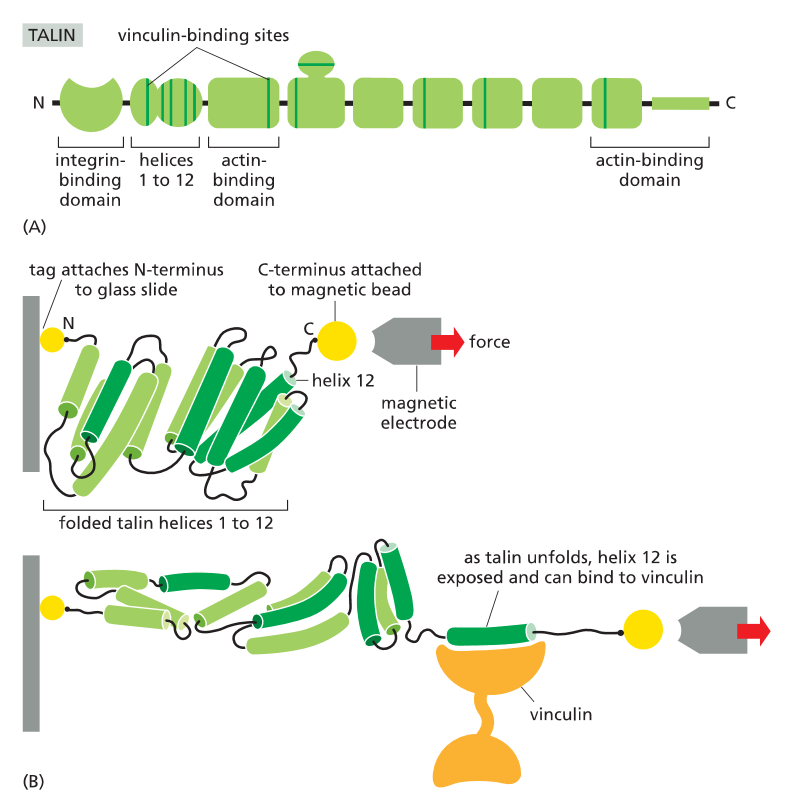
\includegraphics[width=0.6\linewidth]{int_tal}
	\caption{Shows where Talin has different binding domains and how once it gets started to be pulled apart those become uncovered. PSA: this is a pic from an experiment where they used a magnet to pull the molecule apart, we can ignore that.}
	\label{fig:inttal}
\end{figure}

\paragraph{Activation of Integrin Signaling}
Signals received from outside the cell can activate integrin. In \gls{plateletsthrombocytes} (thrombocytes):
\begin{enumerate}
	\item \gls{thrombin} activates a GPCR on the cell surface.
	\item Which in turn activates \gls{Rap1}, a member of the GTPases. It should be said that \textbf{many other receptors can activate Rap1}!
	\item Rap1 interacts with \gls{RIAM}, which then recruits inactive talin and \gls{kindlin} to the membrane surface.
	\item Talin and kindlin interact with the \gls{integrinbeta} to trigger integrin activation.
	\item Talin hangs around to interact with vinculin and more.
\end{enumerate} 

\begin{figure}[H]
	\centering
	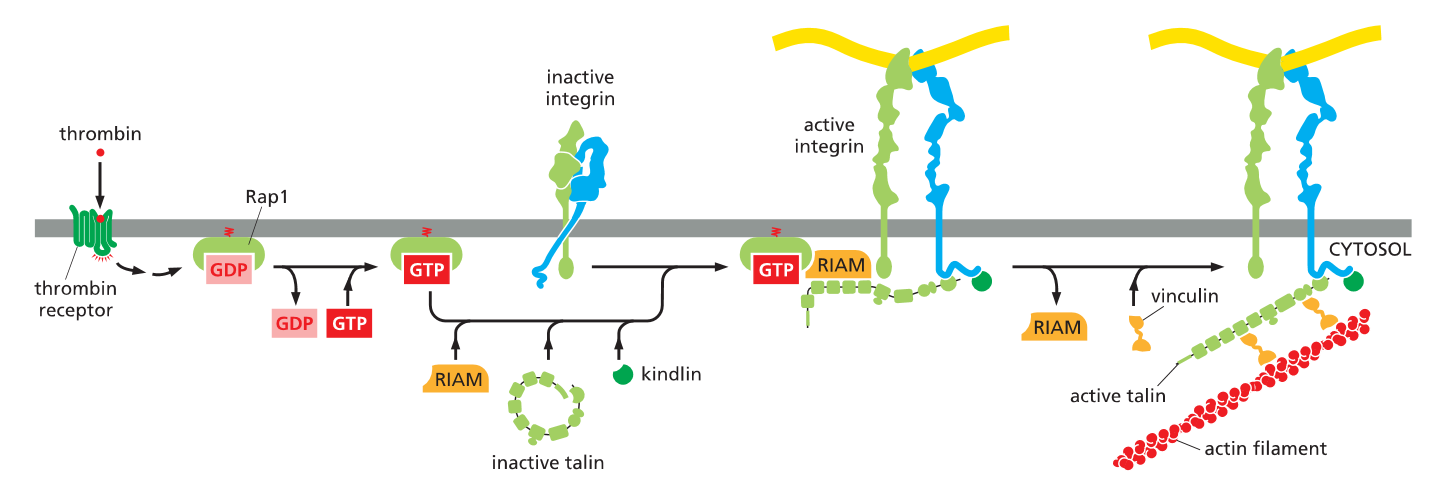
\includegraphics[width=0.9\linewidth]{int_path}
	\caption{The pathway to activate integrin.}
	\label{fig:intpath}
\end{figure}


\begin{RemarkWithTitel}{Talin activation}
	Talin is initially inactive due to a rod domain on the C-terminal and N-terminal which would contain the integrin-binding site but is now blocked. However when RIAM recruits Talin to the membrane, it interacts with a \gls{Phosphoinositide} (PI(4,5)P2) resulting in the dissociation of the \gls{roddomain}. Talin unfolds and binds to integrin.
\end{RemarkWithTitel}

\paragraph{Integrins interacting with the ECM}

Different integrins interact with different components. Arginine-Glycine-Aspartic Acid, RGD are the three amino acids in fibronectin interacting with the integrin $\alpha$5$\beta$1

\begin{figure}[H]
	\centering
	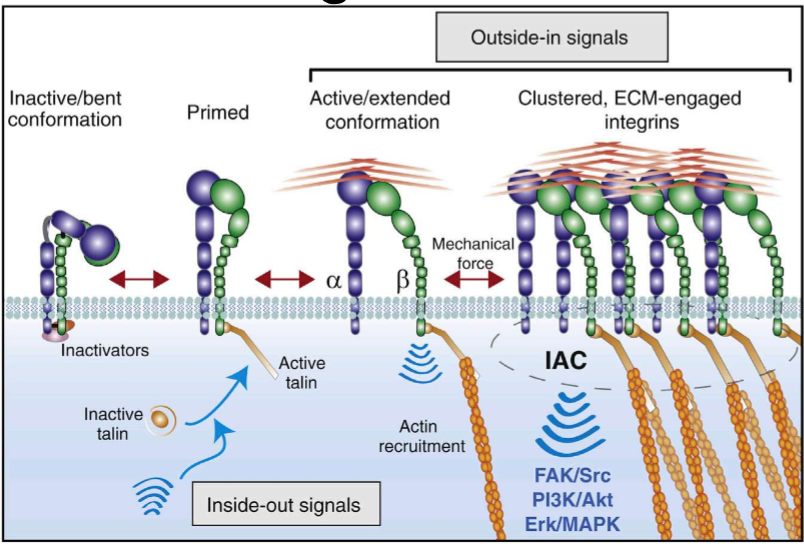
\includegraphics[width=0.5\linewidth]{int_sign}
	\caption{The signal activation and progression from the perspective of integrin.}
	\label{fig:intsign}
\end{figure}


\subsubsection{Laminin}

\gls{Laminin} (\textit{glycoprotein}) is very important for the basal lamina. Due to the binding sites with other proteins, laminin plays a central part in \textbf{organizing and anchoring the basal lamina}. Laminins are multidomain glycoproteins composed of three polypeptide ($\alpha$, $\beta$, $\gamma$), which are bonded through disulfide bonds, bonding them into an asymmetric crosslike structure. Each chain is over 1500 amino acids long. There are 5 $\alpha$, 4 $\beta$, and 3 $\gamma$ different types of chains known to us, which leads to a bunch of different combinations. \gls{Laminin111}, the most understood one, has $\alpha$1, $\beta$1, and you guessed it $\gamma$1 subunits. 

\begin{figure}[H]
	\centering
	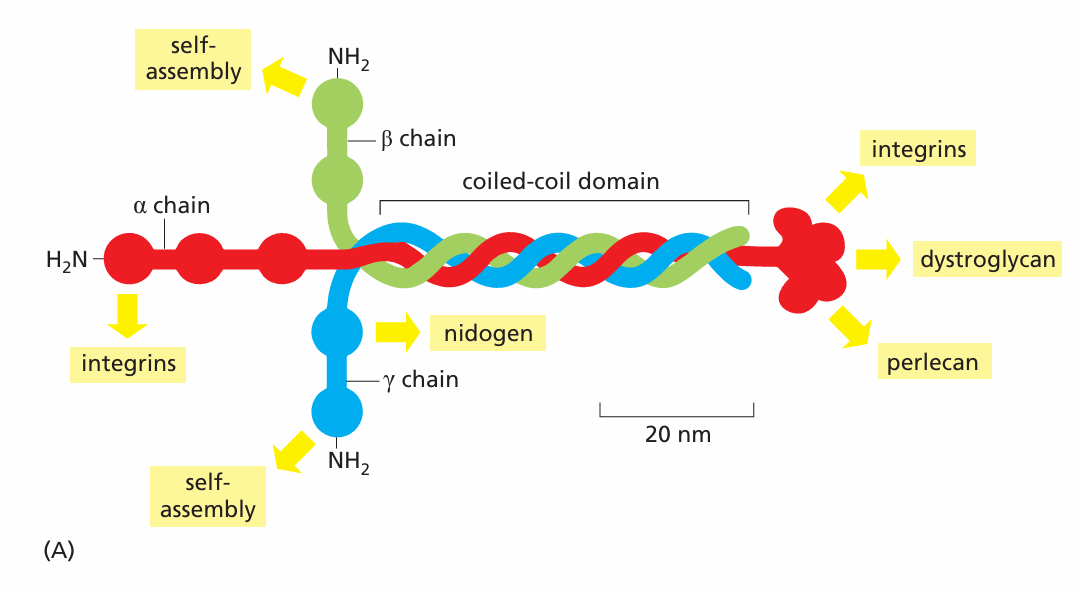
\includegraphics[width=0.7\linewidth]{bl_111}
	\caption{laminin-111, the most understood of laminins, used as example.}
	\label{fig:bl111}
\end{figure}


\subparagraph{The types of laminin}

The \textbf{N-terminus} is responsible for interactions with other extracellular matrix proteins, making it important for the assembly and stability of basement membranes. The \textbf{C-terminus} is responsible for interactions with cell surface receptors, making it crucial for adhesion vs. migration, survival vs. apoptosis, signaling, differentiation, and gene expression. This also shows that \textbf{while the C-terminus is essential, some types laminin don't require a N-terminus}.\\
\\
Here are a bunch of laminin and where they are most commonly found:
\begin{itemize}
	\item 111 mostly in the embryo, rare in adults
	\item 511 and 521 are the most common isoforms in adults
	\item 211 and 221 present in skeletal and cardiac muscles.
	\item 411 and 421 endothelial cells of blood vessels.
	\item 332 is specific for the basal lamina under the epithelial cells (mainly skin).
\end{itemize}

\begin{figure}[H]
	\centering
	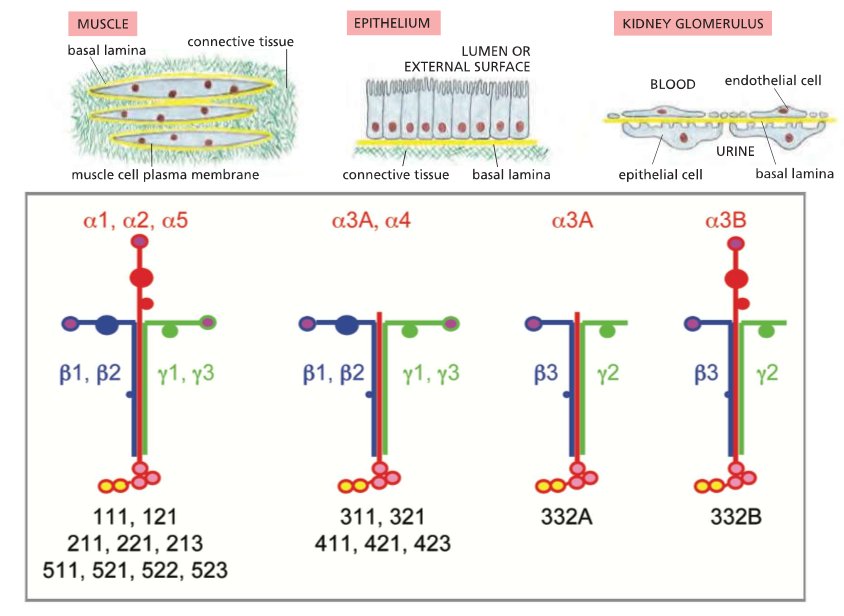
\includegraphics[width=0.6\linewidth]{bl_type}
	\caption{Different groups of laminin and in which types of basal lamina they will mostly be found (laminin looking up is its lamina type).}
	\label{fig:bltype}
\end{figure}


\printglossaries

\end{document}